% **************************** Define Graphics Path **************************
\ifpdf
\graphicspath{{Chapter3/Figs/Raster/}{Chapter3/Figs/PDF/}{Chapter3/Figs/}{Chapter3/Figs/Web/}{Chapter3/Figs/Server/}{Chapter3/Figs/Mobile/}}
\else
\graphicspath{{Chapter3/Figs/Vector/}{Chapter3/Figs/}}
\fi

\chapter{THIẾT KẾ VÀ HIỆN THỰC}
\section{Thiết kế hệ thống}
\subsection{Kiến trúc mô hình hệ thống}\label{sec:struc}
Như đã giới thiệu một số mô hình IoT thực tế ở Mục \ref{sec:xuhuongiot}, mô hình IoT phù hợp mà nhóm sẽ áp dụng cho việc pháp triển hệ thống giám sát được trình bày như Hình \ref{fig:pic5}. Hệ thống bao gồm các thành phần chính như sau: các node cảm biến, trung tâm lưu trữ dữ liệu và ứng dụng truy xuất và hiển thị thông tin phân tích dữ liệu.

\begin{figure}[H]
	\centering    
	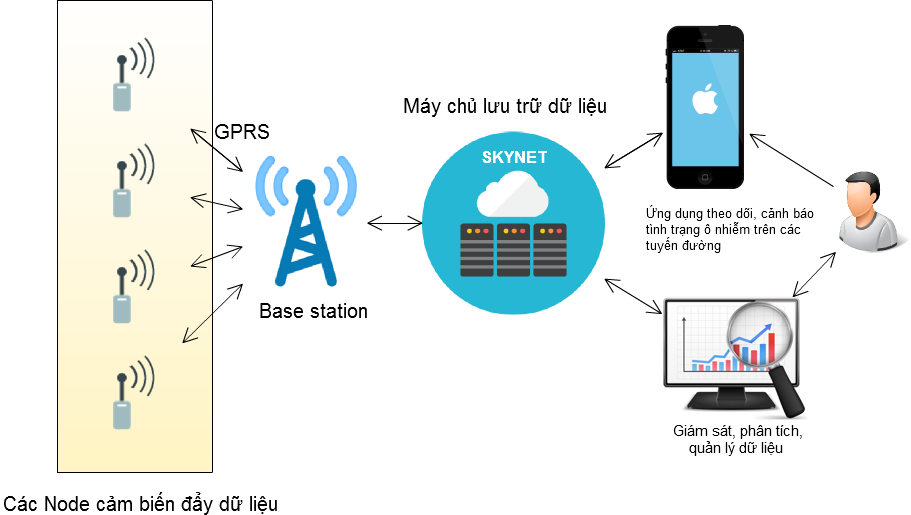
\includegraphics[width=1\textwidth]{system}
	\caption[Kiến trúc mô hình hệ thống]{Kiến trúc mô hình hệ thống}
	\label{fig:system}
\end{figure}

\newpage

\subsection{Các node cảm biến}\label{sec:cacloaicambien}
Các node cảm biến: là một thiết bị được lắp đặt trên những đoạn đường hoặc các địa điểm thích hợp cần để lấy dữ liệu tại khu vực đó, nhiệm vụ chủ yếu là lấy dữ liệu từ các cảm biến đo được sau đó gửi dữ liệu đó lên máy chủ bằng module Sim GPRS.
Để các node cảm biến này được hoạt động dưới tác nhân của môi trường như gió, mưa, bụi, và hơn hết có thể tận dụng nguồn năng lượng mặt trời để nạp pin cho mạch hoạt động độc lập với điện lưới, chúng tôi đã đề xuất mô hình thiết kế node cảm biến để có thể đáp ứng các yêu cầu như sau:
 
\begin{wrapfigure}{l}[4pt]{0.4\linewidth}
    
\includegraphics[scale=0.3]{house_home}
    \caption[Mô hình căn nhà 3D]{Mô hình căn nhà 3D}
    \label{fig:house_home}
\end{wrapfigure}
Lấy ý tưởng từ căn nhà gồm 4 bức tường và 2 mái che như Hình \ref{fig:house_home}, tấm năng lượng mặt trời được thiết kế và gắn như mái che của căn nhà, còn các mạch điện và cảm biến sẽ được đặt bên trong ngôi nhà xung quanh các bức tường được làm từ nhựa mica. Việc lắp đặt node cảm biến này theo hướng các tắm năng lượng mặt trời 1 phía hướng về đông và 1 phía hướng về tây nhằm giúp tắm năng lượng có thể lấy được năng lượng tối đa.

Từ kết quả tìm hiểu các loại khí thải trong mục \ref{sec:yeuto_khithai} đã được nên kết hợp với tình trạng các loại cảm biến hiện có trên thị trường hiện này thì nhóm chúng tôi đã quyết định đưa ra các loại cảm biến cần thiết cho một node cảm biến như sau:



%\\\\\\\\\\\\\\\\\\\\\\\\\\\\\\\\\\\\\\GP2\\\\\\\\\\\\\\\\\\\\\\\\\\\\\\\\\\\\\\\\\\\\%
\subsubsection*{Cảm biến bụi GP2} 
Cảm biến bụi GP2 là một bộ cảm biến chất lượng không khí quang học, được thiết kế đo những hạt bụi. Cám biến được thiết kế một điốt phát hồng ngoại và một photostransistor được sắp xếp thành đường chéo thiết bị này, cho phép nó phát hiện ánh sáng phản xạ của bụi trong không khí.  Nó đặc biệt hiệu quả trong việc phát hiện các hạt rất mịn như khói thuốc lá, và thường được sử dụng trong các hệ thống lọc không khí.

Cảm biến bụi GP2 tiêu tốn dòng rất ít (20 mA cao nhất, 11mA chế độ chạy thường), có thể hỗ trợ nguồn cung cấp lên tới 7VDC. Tín hiệu đầu ra của cảm biến là dạng tín hiệu tương tự dùng để đo mật độ bụi, với độ nhạy $0.5V/0.1mg/{m}^{3}$.

Thông số kỹ thuật:
\begin{itemize}
\item[•]Nguồn hoạt động: 5VDC
\item[•]Dòng tiêu thụ: 10mA
\item[•]Ngõ ra analog
\item[•]Nhiệt độ hoạt động: $-40^{o}$ $-$ $85 ^{o}$ C
\end{itemize}

\begin{figure}[H]
	\centering    
	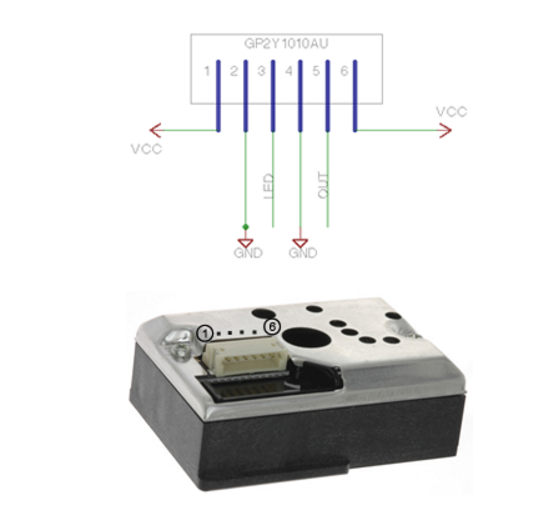
\includegraphics[width=0.5\textwidth]{gp2}
	\caption[Cảm biến bụi GP2 ]{Cảm biến bụi GP2}
	\label{fig:gp2}
\end{figure}

Sơ đồ kết nối cảm biến bụi GP2 với Arduino
Theo hướng dẫn của tài liệu kỹ thuật, nó có tất cả gồm 6 chân đầu ra để kết nối tới thiết bị. Để có thể cảm biến bụi GP2 hoạt động với vi xử lý Arduino cần kết nối như sơ đồ luận lý sau:

\begin{figure}[H]
	\centering    
	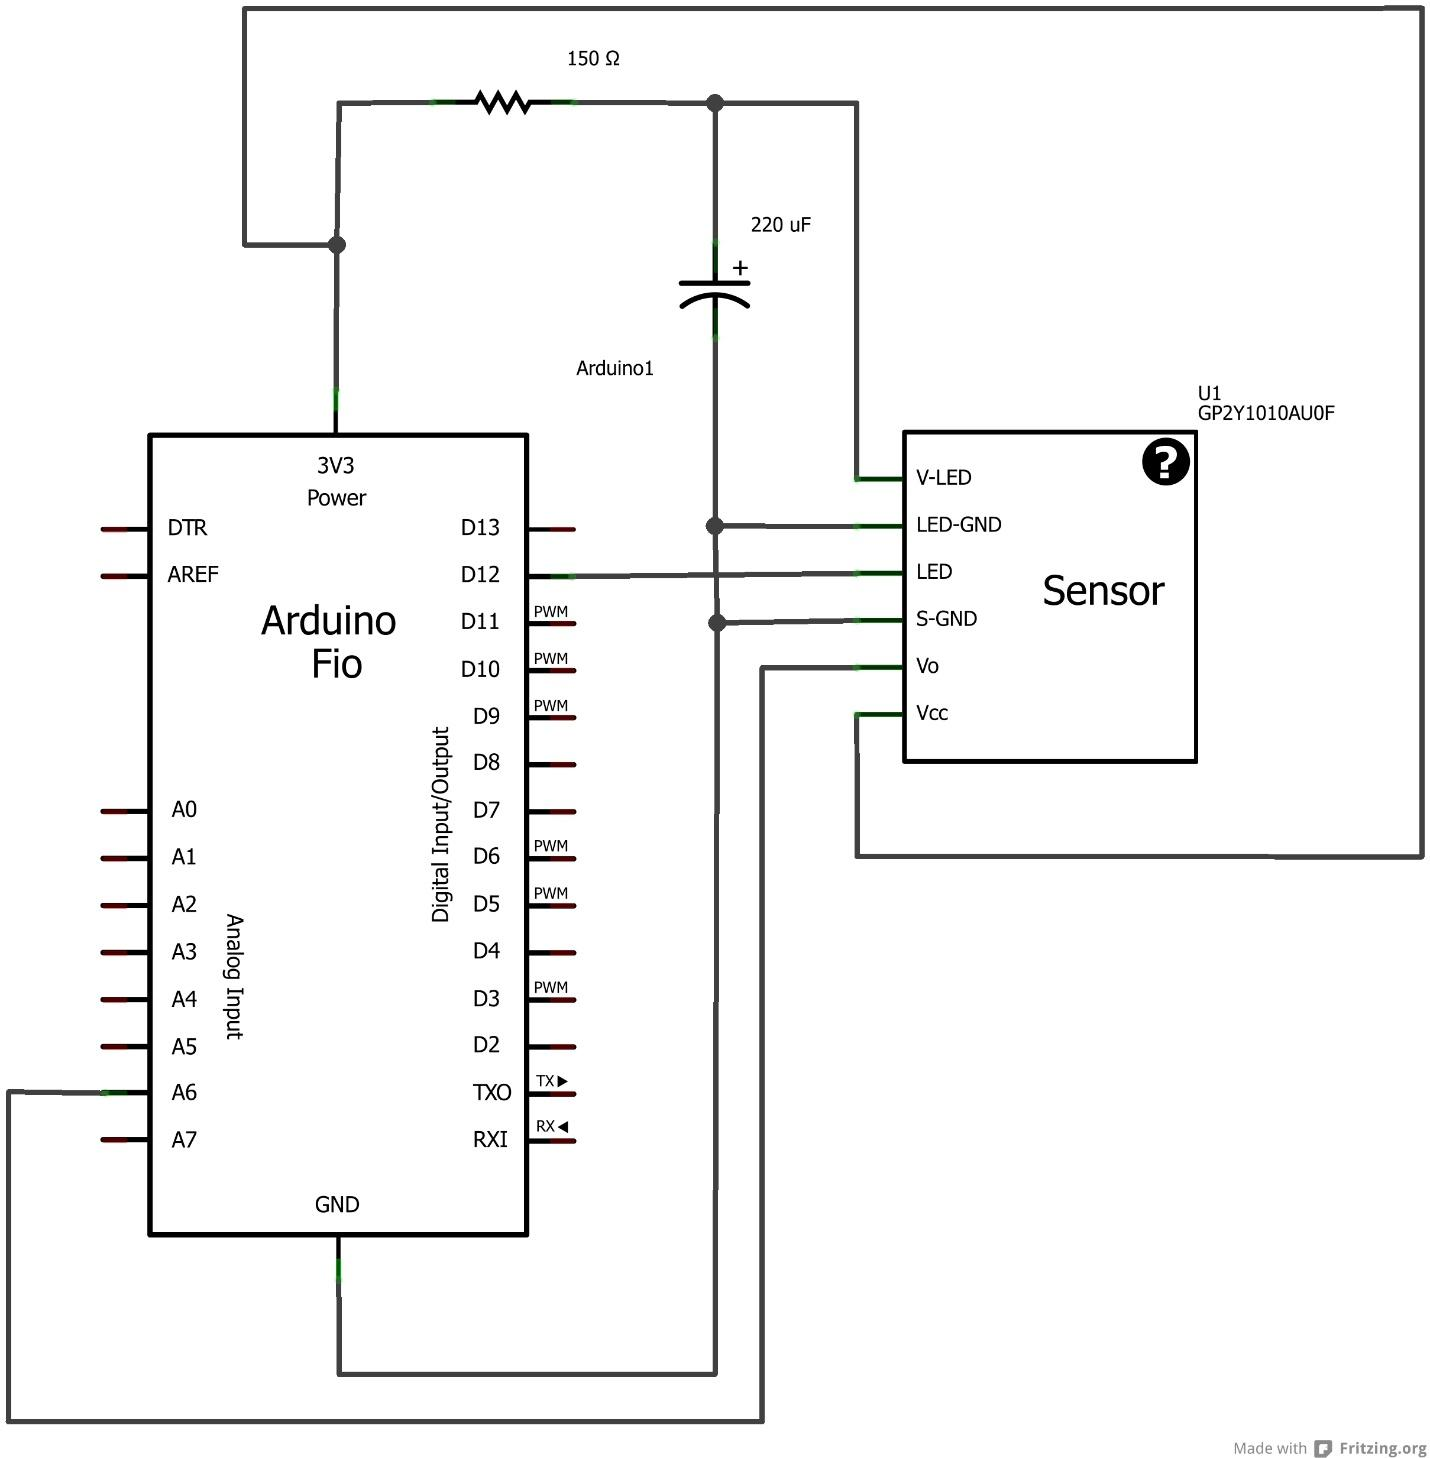
\includegraphics[width=0.7\textwidth]{sodogp2}
	\caption[Sơ đồ GP2 kết nối với Arduino ]{Sơ đồ GP2 kết nối với Arduino}
	\label{fig:sodogp2}
\end{figure}






%\\\\\\\\\\\\\\\\\\\\\\\\\\\\\\\\\\\\\\	MQ135	\\\\\\\\\\\\\\\\\\\\\\\\\\\\\\\\\\\\\\\\\\\\%
\newpage
\subsubsection*{Cảm biến chất lượng không khí MQ135} 
Cảm biến chất lượng không khí MQ135 thường được dùng trong các thiết bị kiểm tra chất lượng không khí bên trong cao ốc, văn phòng, thích hợp để phát hiện khí NH3, Nox, Ancol, Benzen, khói và khí CO2.Cám biến này với độ nhạy cao và thời gian đáp ứng nhanh. Tín hiệu ngõ ra dạng analog và digital. Cảm biến này có thể hoạt động ở nhiệt độ từ khoảng: $-10^{o}$C đến $50^{o}$C và tiêu thụ dòng khoảng 300mA tại 5V.
\begin{figure}[H]
	\centering    
	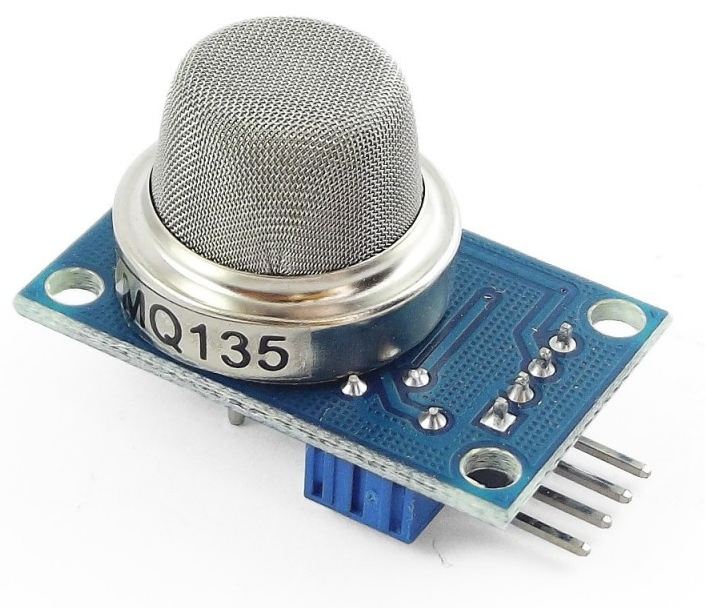
\includegraphics[width=0.7\textwidth]{mq135}
	\caption[Cảm biến MQ135]{Cảm biến MQ135}
	\label{fig:mq135}
\end{figure}
Thông số kỹ thuật:
\begin{itemize}
\item[•]Điện áp cung cấp: <=24 VDC
\item[•]Điện áp heater: 5V AC/DC
\item[•]Sử dụng chip so sánh LM393c.
\item[•]Hai tín hiệu đầu ra (digital và analog)
\item[•]Tín hiệu analog từ 0 ~ 5V.
\item[•]Dải phát hiện từ 10 đến 1000ppm
\end{itemize}

\begin{figure}[H]
	\centering    
	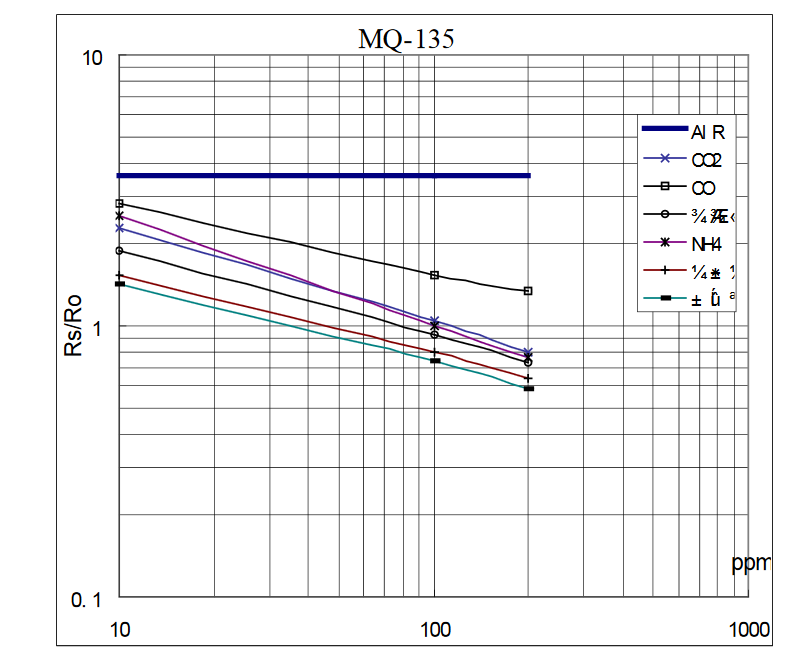
\includegraphics[width=0.7\textwidth]{mq135_mqh1}
	\caption[Giản đồ chỉ sự biến đổi của Rs/Ro và giá trị ppm của MQ135]{Giản đồ chỉ sự biến đổi của Rs/Ro và giá trị ppm của MQ135}
	\label{fig:mq135_mqh1}
\end{figure}

\begin{figure}[H]
	\centering    
	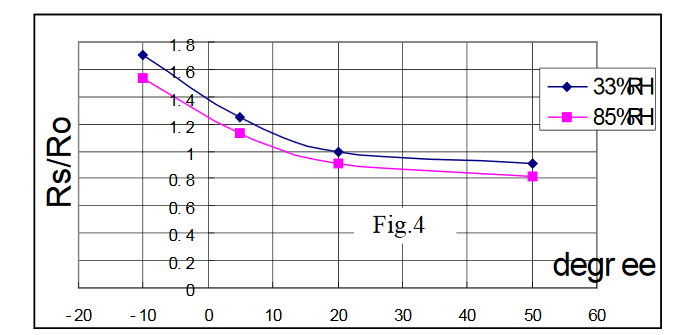
\includegraphics[width=0.7\textwidth]{mq135_mqh2}
	\caption[Giản đồ chỉ sự biến đổi của Rs/Ro đối với nhiệt độ, độ ẩm]{Giản đồ chỉ sự biến đổi của Rs/Ro đối với nhiệt độ, độ ẩm}
	\label{fig:mq135_mqh2}
\end{figure}


Giá trị chất lượng không khí(ppm) được xác định theo biểu đồ Hình \ref{fig:mq135_mqh1} giá trị này thay đổi theo sự biến đổi của giá trị Rs/Ro, theo Hình \ref{fig:mq135_mqh2} thì giá trị Rs/Ro bị ảnh hưởng bởi nhiệt độ và độ ẩm.

Để xác định được giá trị Rs/Ro từ ngõ ra analog của mạch cảm biến MQ-135 ta có công thức như sau:
\begin{center}
$\displaystyle \frac{R_{S}}{R_{L}} = \frac{V_{C}-V_{RL}}{V_{RL}}$
\end{center}

Giá trị Rs/Ro này được vi xử lý tính toán dựa trên đầu ra analog của cảm biến MQ-135 và được đưa vào thư viện mq135.h để có thể lấy được giá trị chất lượng không khí ppm theo sự thay đổi của nhiệt độ và độ ẩm của môi trường thực tế.

Thư viện mq135.h cung cấp cho chúng ta các hàm toán học đã được nhà sản xuất tính toán sẵn để có thể lấy được giá trị chất lượng không khí ppm dựa vào thay đổi của môi trường nhiệt độ và độ ẩm.



%\\\\\\\\\\\\\\\\\\\\\\\\\\\\\\\\\\\\\\	MQ07	\\\\\\\\\\\\\\\\\\\\\\\\\\\\\\\\\\\\\\\\\\\\%
\newpage
\subsubsection*{Cảm biến chất lượng không khí MQ07} 
Cảm biến khí CO MQ-7 có thể pháp hiện khí CO tập trung ở những nơi khác nhau từ 10 đến 1000ppm. Cám biến này với độ nhạy cao và thời gian đáp ứng nhanh. Tín hiệu ngõ ra dạng analog và digital. Cảm biến này có thể hoạt động ở nhiệt độ từ khoảng: -10C đến 50C và tiêu thụ dòng khoảng 250mA tại 5V.
\begin{figure}[H]
\centering    
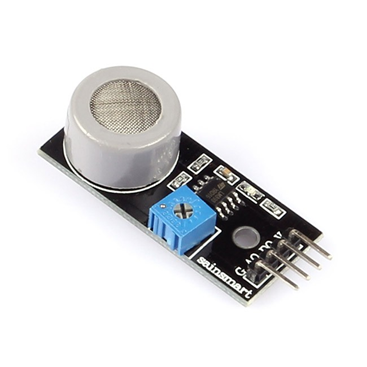
\includegraphics[width=0.7\textwidth]{mq07}
\caption[Cảm biến MQ07]{Cảm biến MQ07}
\label{fig:mq07}
\end{figure}


Thông số kỹ thuật:
\begin{itemize}
\item[•]Điện áp cung cấp: 3 ~ 5VDC.
\item[•]Sử dụng chip so sánh LM393 và MQ-7.
\item[•]Hai tín hiệu đầu ra (digital và analog)
\item[•]Tín hiệu analog từ 0 ~ 5V.
\item[•]Dải phát hiện từ 10 đến 1000ppm
\item[•]Kích thước: 33 x 20 x 16mm.
\end{itemize}
\begin{figure}[H]
\centering    
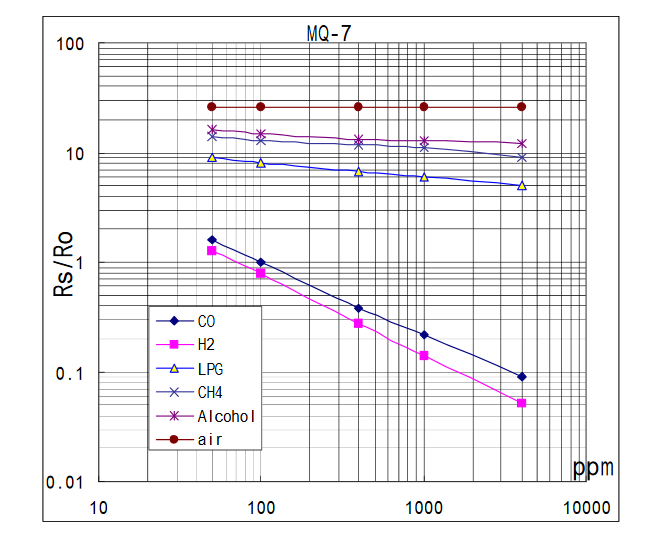
\includegraphics[width=0.7\textwidth]{mq07_mqh1}
\caption[Giản đồ chỉ sự biến đổi của Rs/Ro và giá trị ppm của MQ07]{Giản đồ chỉ sự biến đổi của Rs/Ro và giá trị ppm của MQ07}
\label{fig:mq07_mqh1}
\end{figure}


\begin{figure}[H]
\centering    
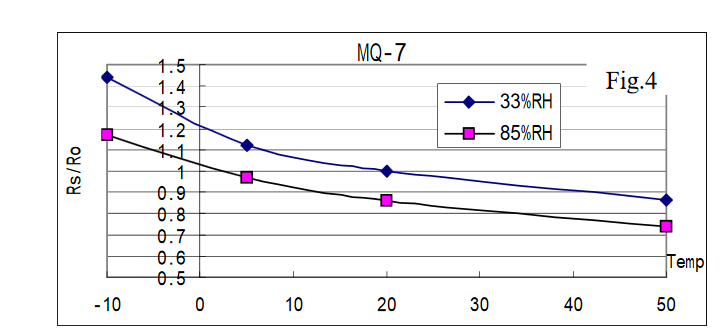
\includegraphics[width=0.7\textwidth]{mq07_mqh2}
\caption[Giản đồ chỉ sự biến đổi của Rs/Ro đối với nhiệt độ, độ ẩm]{Giản đồ chỉ sự biến đổi của Rs/Ro đối với nhiệt độ, độ ẩm}
\label{fig:mq07_mqh2}
\end{figure}


Giá trị chất lượng không khí(ppm) được xác định theo biểu đồ Hình \ref{fig:mq07_mqh1} giá trị này thay đổi theo sự biến đổi của giá trị Rs/Ro, theo Hình \ref{fig:mq07_mqh2} thì giá trị Rs/Ro bị ảnh hưởng bởi nhiệt độ và độ ẩm.

Để xác định được giá trị Rs/Ro từ ngõ ra analog của mạch cảm biến MQ-7 ta có công thức như sau:
\begin{center}
$\displaystyle \frac{R_{S}}{R_{L}} = \frac{V_{C}-V_{RL}}{V_{RL}}$
\end{center}

Giá trị Rs/Ro này được vi xử lý tính toán dựa trên đầu ra analog của cảm biến MQ-7 và được đưa vào thư viện mq07.h để có thể lấy được giá trị chất lượng không khí ppm theo sự thay đổi của nhiệt độ và độ ẩm của môi trường thực tế.

Thư viện mq07.h cung cấp cho chúng ta các hàm toán học đã được nhà sản xuất tính toán sẵn để có thể lấy được giá trị chất lượng không khí ppm dựa vào thay đổi của môi trường nhiệt độ và độ ẩm.






%\\\\\\\\\\\\\\\\\\\\\\\\\\\\\\\\\\\\\\	Cảm biến nhiệt độ DS18B20 IC	\\\\\\\\\\\\\\\\\\\\\\\\\\\\\\\\\\\\\\\\\\\\%
\newpage
\subsubsection*{Cảm biến nhiệt độ DS18B20 IC} 
Cảm biến nhiệt độ DS18B20 là cảm biến loại tín hiệu đầu ra digital đo nhiệt độ mới của hãng MAXIM với độ phân giải cao (12bit). IC được sử dụng giao tiếp 1 dây rất gọn gàng, dễ lập trình và giao tiếp nhiều DS18B20 trên cùng 1 dây. IC còn có chức năng cảnh báo nhiệt độ khi vượt ngưỡng và đặc biệt hơn là có thể cấp nguốn từ chân data.

\begin{figure}[H]
	\centering    
	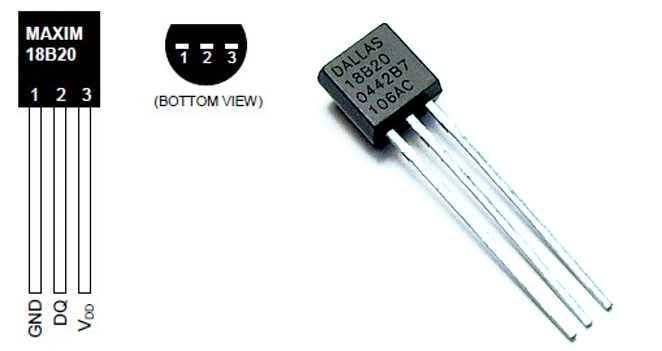
\includegraphics[width=0.7\textwidth]{ds18b20}
	\caption[Cảm biến nhiệt độ DS18B20]{Cảm biến nhiệt độ DS18B20}
	\label{fig:ds18b20}
\end{figure}

Thông số kỹ thuật:
\begin{itemize}
\item[•]Nguồn: 3-5.5V
\item[•]Dải đo nhiệt độ: -55 -125 * C
\item[•]Sai số: +-0.5 *C
\item[•]Độ phân giải: 9-12bits
\item[•]Thời gian chuyển đổi nhiệt độ: 750ms
\end{itemize}
Sơ đồ kết nối IC BS18B20 để lấy được tín hiệu data
\begin{figure}[H]
	\centering    
	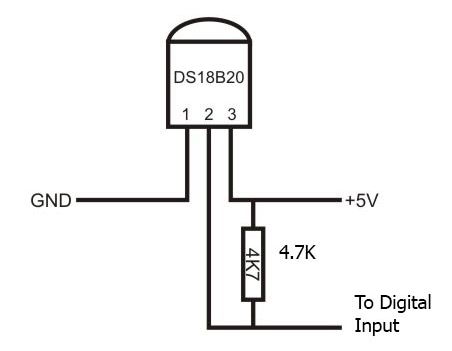
\includegraphics[width=0.7\textwidth]{ds18b20_ketnoi}
	\caption[Sơ đồ kết nối DS18B20]{Sơ đồ kết nối DS18B20}
	\label{fig: ds18b20_ketnoi}
\end{figure}
Chân Digital input sẽ được đưa tới chân Digital input của board arduino nano, hiện tại nhà sản xuất cũng cung cấp cho lập trình viên về bộ thư viện để có thể sử dụng trong việc phát triển.

\newpage


\subsection{Chuẩn giao tiếp giữa các node tới máy chủ}
Để các node cảm biến gửi dữ liệu lên máy chủ thì chúng tôi đã sử dụng module Sim800L được giới thiệu trong mục \ref{sec:sim800l}. Quá trình kết nối của các node cảm biến tới máy chủ thông qua giao thức TCP được thực hiện dựa trên mô hình máy trạng thái như sau:


\begin{figure}[H]
\centering   
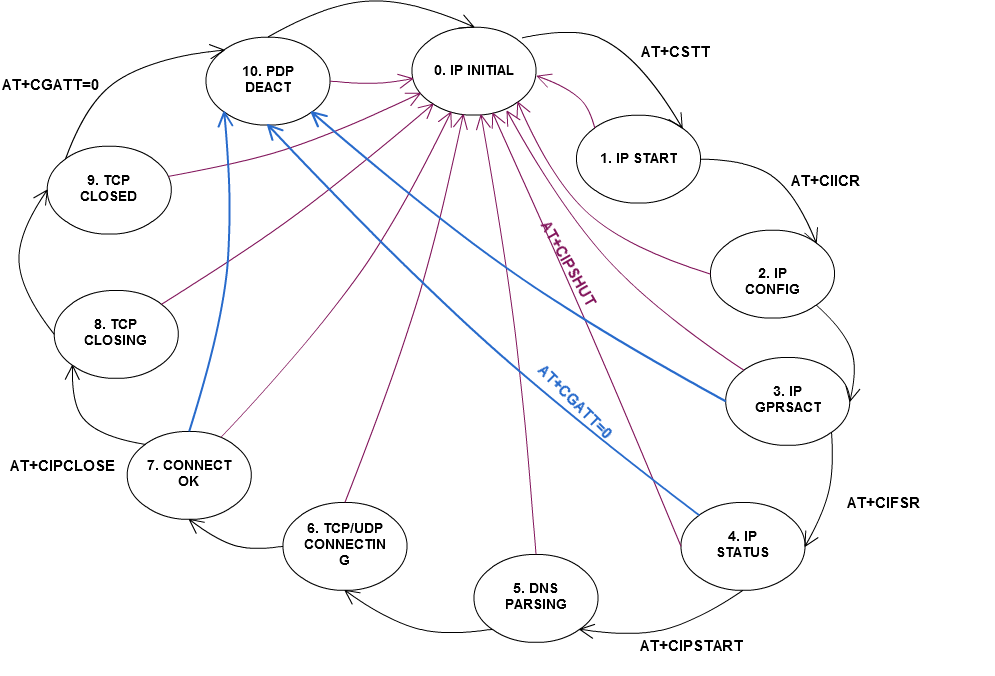
\includegraphics[width=1\textwidth]{sim800_status}
\caption[Sơ đồ trạng thái GPRS cho đơn kết nối]{Sơ đồ trạng thái GPRS cho đơn kết nối}
\label{fig:sim800_status}
\end{figure}

Để gửi được dữ liệu đến máy chủ cần phải thiết lập được kết nối TCP từ module SIM800 đến máy chủ thông qua 11 trạng thái như Hình \ref{fig:sim800_status}, các trạng thái được chuyển đổi thông qua các tập lệnh AT đã được đề cập tại mục \ref{sec:sim800l}. Đến trạng thái 7 (CONNET OK) chúng ta đã giữ được kết nối TCP tới máy chủ và tại trạng thái này dùng lệnh AT+CIPSEND để thực hiện việc gửi gói dữ liệu lên cho máy chủ.

Gói dữ liệu được gửi theo phương thức GET, bên máy chủ phải hỗ trợ được phương thức GET này và định nghĩa rõ ràng các kiểu và số lượng dữ liệu gửi lên. 

Dữ liệu sensor node gửi lên cho máy chủ gồm các dữ liệu sau:
\begin{table}[]
\centering
\label{table:sensornode_api}
\begin{tabular}{|l|l|l|l|l|l|}
\hline
\begin{tabular}[c]{@{}l@{}}NODE\\ ID\end{tabular} & \begin{tabular}[c]{@{}l@{}}Giá trị CO\\ (ppm)\end{tabular} & \begin{tabular}[c]{@{}l@{}}Giá trị \\ nhiệt độ \\ (Độ C)\end{tabular} & \begin{tabular}[c]{@{}l@{}}Giá trị\\ độ bụi\\ (ppm)\end{tabular} & \begin{tabular}[c]{@{}l@{}}Giá trị chất\\ lượng không \\ khí (ppm)\end{tabular} & \begin{tabular}[c]{@{}l@{}}Giá trị dung\\ lượng pin (\%)\end{tabular} \\ \hline
\end{tabular}
\end{table}
\subsection{Thiết kế API}\label{sec: api}
Mục tiêu đề tài không chỉ thu thập và thống kê mà còn chia sẻ dữ liệu. Để làm được điều đó thì cần phải có API cung cấp cho những nhà phát triển thứ 3, có thể dùng API được cung cấp để sử dụng dữ liệu để phát triển. Bởi vì vậy hệ thống có xây dựng hệ thống API mở.

Ở bảng \ref{table: apilist}, hệ thống cung cấp các API về quản lý và truy vấn dữ liệu của các sensor node. Sử dụng hai method POST và GET để gửi request tới Server. 

\begin{table}[H]
	\centering
	\caption{Bảng API tương tác với dữ liệu về các node}
	\begin{tabular}{|l|l|l|l|}
		\hline
		Method & URL            & Miêu tả         & Yêu cầu xác thực người dùng        \\ \hline
		POST   & /node/initnew       & Khởi tạo node mới                & Có           \\ \hline
		POST   & /node/updatenode     & Cập nhật thông tin node & Có \\ \hline
		POST   & /node/replacenode       & Thay thế node  & Có       \\ \hline
		GET   & /node/pushdata & Push dữ liệu               &         Không                \\ \hline
		GET   & /node/getdata    & Get dữ liệu thu thập của node         &  Không      \\ \hline
		GET   & /node/getinfo   & Get thông tin của node & Không  \\ \hline
	\end{tabular}
	\label{table: apilist}
\end{table}

Giao thức được lựa chọn sử dụng trong việc push data là giao thức HTTP mà không phải các giao thức thuần để phát triển IoT như MQTT hay CoAp vì tính phổ biến và dễ thiết lập sử dụng. Chỉ cần thiết lập chuỗi URL có đính kèm thông tin là có thể hòa nhập với hệ thống mà không cần thiết lập gì thêm, có thể ví như là "plug and play" vì tính đơn giản và hoạt động với mọi thiết bị có hỗ trợ kết nối Internet.

Bù lại, so với các giao thức tối ưu dung lượng gói tin cho phát triển IoT như MQTT, gói tin gửi qua HTTP có dung lượng nhiều hơn đáng kể nhưng với tần số hoạt động truyền dữ liệu của đề tài thì vẫn có thể chấp nhận được và không tạo ra sự khác biệt lớn khi hoạt động.

Về phần API trợ giúp đăng ký và xác thực người dùng được quy ước như bảng \ref{table: apiuser}.
\begin{table}[H]
	\centering
	\caption{Bảng API tương tác với dữ liệu về các node}
	\begin{tabular}{|l|l|l|}
		\hline
		Method & URL            & Miêu tả                \\ \hline
		POST   & /auth/login       & Đăng nhập                           \\ \hline
		GET   & /auth/logout   & Đăng xuất   \\ \hline
		POST   & /user/register     & Đăng ký người dùng mới \\ \hline
	\end{tabular}
	\label{table: apiuser}
\end{table}
\subsection{Cách thức tương tác cập nhật dữ liệu}

Trong việc tương tác cập nhật dữ liệu, hiện nay mô hình truy thường được sử dụng là \textbf{polling}. Client và server phải liên tục gửi các request liên tục cách nhau trong một thời gian cố định để kiểm tra liệu có sự thay đổi cập nhật dữ liệu. 
\begin{figure}[H]
	\centering    
	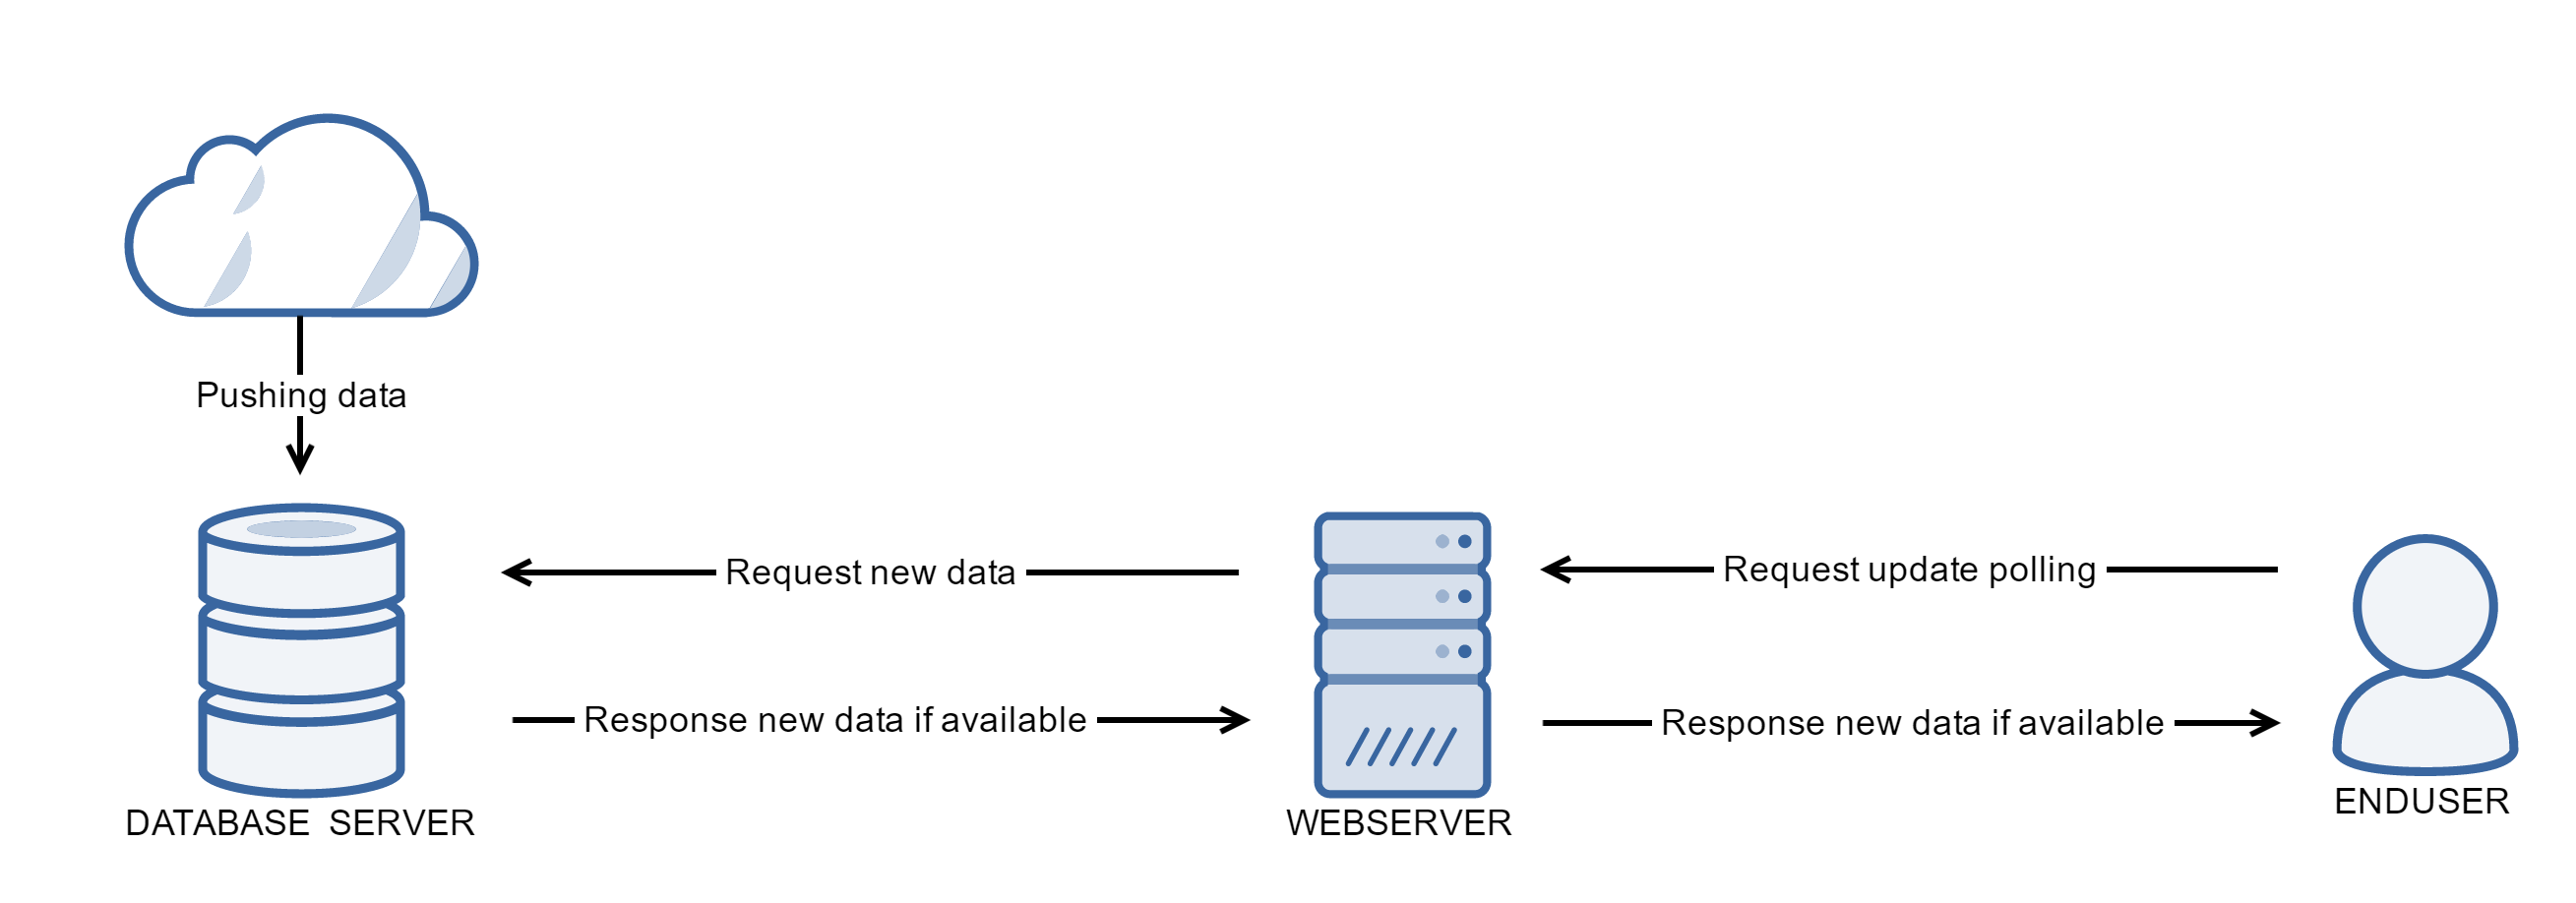
\includegraphics[width=1.0\textwidth]{polling}
	\caption[Mô hình tương tác polling]{Mô hình tương tác polling}
	\label{fig: polling}
\end{figure}
Phương pháp này dễ hiện thực và áp dụng, tuy nhiên sẽ mắc nhược điểm là tốn nhiều gói tin request vô dụng làm giảm hiệu năng hệ thống, và không đáp ứng tính realtime nếu như chu kì gửi request dài.



Vì hiện tại nhóm chúng tôi đang hướng tới hướng phát triển IoT, đòi hỏi yêu cầu về tính realtime cũng như tối ưu hóa hệ thống. Và để đáp ứng yêu cầu đó, nhóm đã tìm tới giải pháp giữ socket kết nối từ \textbf{Database} (RethinkDB) <-> \textbf{Server} (Chạy trên nền tảng Nodejs) <-> \textbf{Client} (web browser)

\begin{figure}[H]
	\centering    
	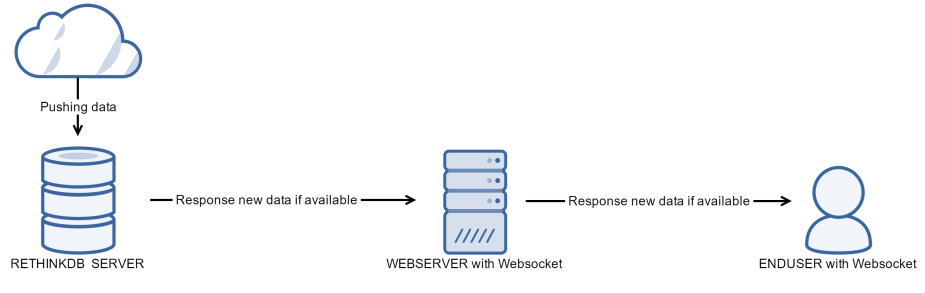
\includegraphics[width=1.0\textwidth]{realtime}
	\caption[Mô hình tương tác realtime dựa trên Socket]{Mô hình tương tác realtime dựa trên Socket}
	\label{fig: realtime}
\end{figure}

Như hình \ref{fig: realtime}, mô hình hoạt động đơn giản hơn rất nhiều, giảm bớt số lượng request không đáng có và đảm bảo tính realtime cho hệ thống.

Một điểm mạnh ở mô hình này nữa là có thể phát triển nhiều server hoặc ứng dụng di động sử dụng chung một hệ quản lý cơ sở dữ liệu nhưng vẫn đảm bảo sự đồng bộ dữ liệu cập nhật tới enduser theo thời gian thực.
\begin{figure}[H]
	\centering    
	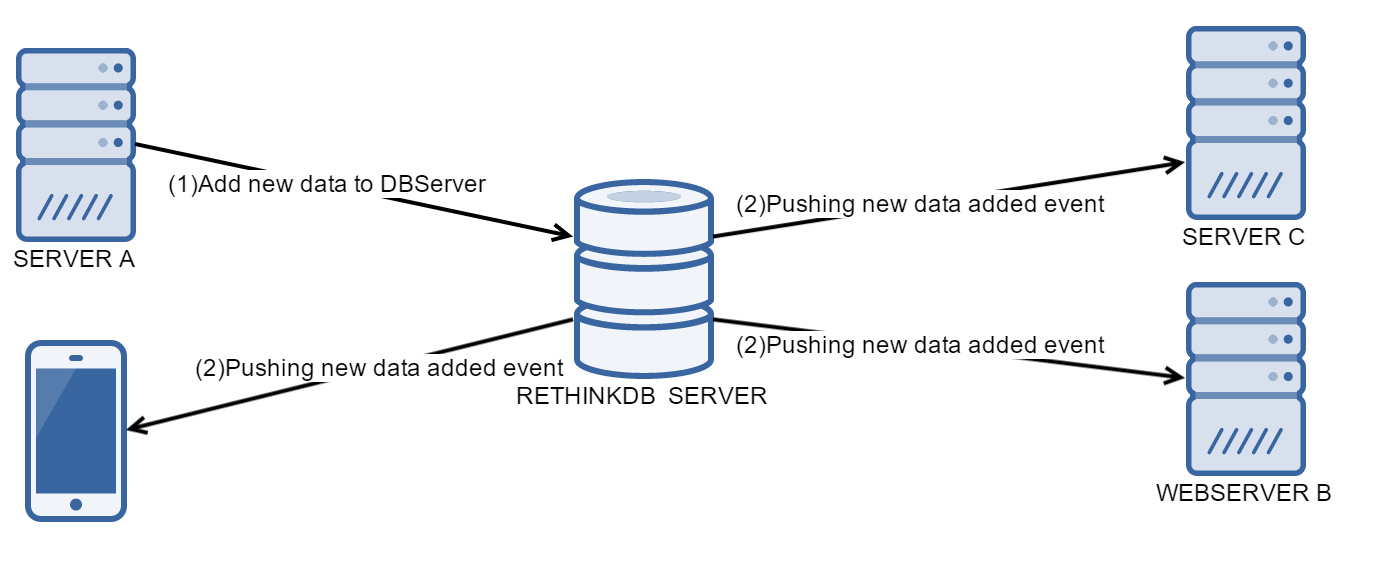
\includegraphics[width=1.0\textwidth]{multiserver}
	\caption[Mô hình tương tác cập nhật nhiều Server]{Mô hình tương tác cập nhật nhiều Server và Client}
	\label{fig: multiserver}
\end{figure}
\subsection{Mô hình ứng dụng trình bày dữ liệu}
\subsubsection*{Chức năng Web Server}
Đối với người dùng:
\begin{itemize}
\item[•] Cung cấp cho người dùng thông tin về nơi chứa node cảm biến.
\item[•] Người dùng có thể xem biểu đồ dữ liệu thông số môi trường tại vị trí tương ứng với node cảm biến đã được thiết lập.
\item[•] Xem được tình trạng và biểu đồ thống kê của các node cảm biến đang hoạt động.
\item[•] Gửi phản thông tin phản hồi về cho người quản lý thông qua email.
\item[•] Cung cấp thông tin lịch sử các hoạt động sử dung API, giúp cho bên thứ 3 có thể dễ dàng phát triển.
\end{itemize}

Đối với người quản lý:
\begin{itemize}
\item[•] Bao gồm tất cả chức năng của người dùng bình thường.
\item[•] Quản lý chỉnh sửa thông tin các node cảm biến: thêm, xóa, cập nhật, thay đổi.
\end{itemize}

\subsubsection*{Biểu đồ High level Usecase của Web Server}

\begin{figure}[H]
\centering    
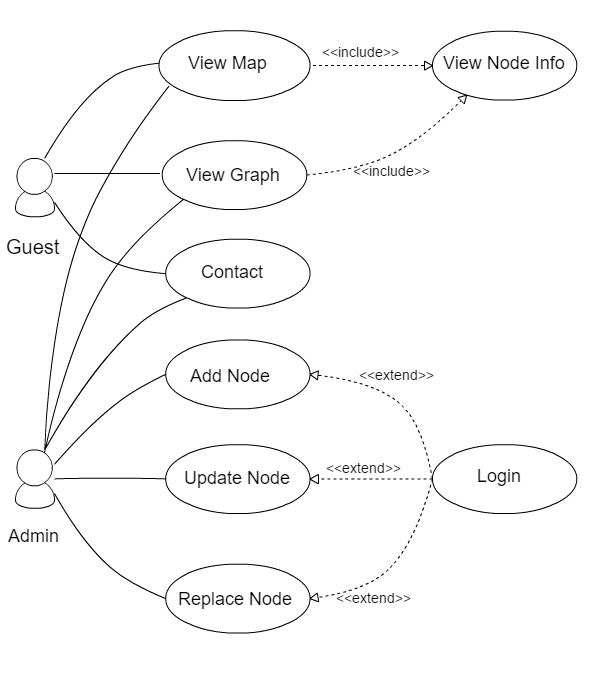
\includegraphics[width=0.7\textwidth]{usecase_diagram}
\caption[Biểu đồ High level Usecase]{Biểu đồ High level Usecase }
\label{fig:usecase_diagram}
\end{figure}

Mô tả giản đồ Usecase

\begin{table}[]
\centering
\caption{Bảng mô tả giản đồ Usecase của Web Server}
\label{my-label}
\begin{tabular}{|l|l|l|}
\hline
STT & Tên            & Miêu tả                                                                                            \\ \hline
1   & View map       & Người dùng thấy được các node đang chạy trên google maps                                           \\ \hline
2   & View Node Info & Thông tin tương ứng của Node( Lat, Lng, Phone)                                                     \\ \hline
3   & View Graph     & \begin{tabular}[c]{@{}l@{}}Đồ thị hoạt động của Node(các số liệu đo được theo\\ ngày)\end{tabular} \\ \hline
4   & Contact        & Phản hồi ý kiến người dùng qua Gmail                                                               \\ \hline
5   & Add Node       & Thêm mới Node vào hoạt động                                                                        \\ \hline
6   & Update Node    & Thay đổi thông tin của Node( Lat, Lng, Phone)                                                      \\ \hline
7   & Replace Node   & Thay đổi 1 Node xảy ra sự cố bằng 1 Node khác                                                      \\ \hline
\end{tabular}
\end{table}




%%%%%%%%%%%%%%%%%%%%%%%%%%%%%%%%%%%%%%%%%%%%%%%%%%%%%%%%%%%%%%%%%%%%%%%%%%
% 				VẼ MẤY CÁI D.	Acitivity diagram VÀO ĐÂY %%%%%%%%%%%%%%%%%
%%%%%%%%%%%%%%%%%%%%%%%%%%%%%%%%%%%%%%%%%%%%%%%%%%%%%%%%%%%%%%%%%%%%%%%%%%%%%




\subsubsection*{Chức năng Ứng dụng di động}
Hiện thị thông tin các node cảm biến đang hoạt động qua màn hình chính, và biểu đồ dữ liệu của từng node cảm biến theo từng ngày, thêm sự kết nối với web browser tạo sự thuận tiện cho việc theo dõi, hiện thị đồ thị (2 kiểu đồ thị là line chart và bar chart).
\subsubsection*{Biểu đồ High level Usecase của ứng dụng di động}

\begin{figure}[H]
\centering    
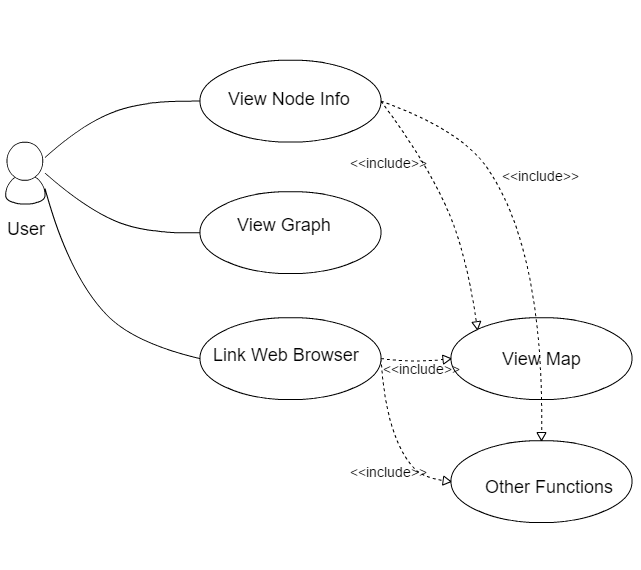
\includegraphics[width=0.7\textwidth]{app_usecase}
\caption[Giản đồ High level Usecase của ứng dụng di động]{Giản đồ High level Usecase của ứng dụng di động}
\label{fig:app_usecase}
\end{figure}

Mô tả Usecase

\begin{table}[H]
\centering
\caption{Bảng mô tả giản đồ Usecase của ứng dụng di động}
\label{table:usecase_mobile}
\begin{tabular}{|l|l|l|}
\hline
STT & Tên Use-case     & Mô tả                                                            \\ \hline
1   & View Node Info   & Thông tin của Node( Lat, lng, Phone, ID)                         \\ \hline
2   & View Graph       & 2 dạng đồ thị theo ngày (line chart, bar chart của các thông số) \\ \hline
3   & Link web browser & Liên kết tới web browser                                         \\ \hline
4   & View Map         & Hiện thị Google Map và vị trí các Node                           \\ \hline
5   & Other Functions  & Các chức năng của web browser                                    \\ \hline
\end{tabular}
\end{table}













\subsection{Các ràng buộc của hệ thống}
Cũng như các dự án IoT quy mô rộng khác, đề tài cũng yêu cầu nhiều đặc tính ràng buộc như:  
\subsubsection*{Tính đáp ứng thời gian thực}Để giải quyết tình trạng giao thông hiện thời và trong thời gian gần, ta cần phải có dữ liệu thời gian thực. Ta không thể sử dụng dữ liệu của nửa tiếng hoặc 1 giờ trước để vẽ nên bản đồ lưu thông hiện tại cũng như cách điều hướng giải quyết. Do đó, hệ thống cần phải có thời gian đáp ứng nhanh khi có yêu cầu dữ liệu khi được gọi. Để đạt được kết quả đó, ta cần phải có những phần cứng với thiết lập kết nối có khả năng đáp ứng nhanh, cùng với khả năng hoạt động ổn định liên tục trong thời gian dài để cung cấp dữ liệu liên tục và liền mạch.


\subsubsection*{Toàn vẹn dữ liệu (Data Integrity)} Mục đích chính của dự án là thu thập dữ liệu và từ đó phát triển ứng dụng. Vì thế tính toàn vẹn dữ liệu đóng vai trò quan trọng. Dữ liệu thu thập cần phải đáp ứng đủ các yếu tố: tin cậy, chính xác và đầy đủ. Ta cần phải có đủ dữ liệu thì mới có thể đủ dữ kiện để giải quyết bài toán. Ta không thể giải quyết khi chỉ có được dữ liệu một đoạn đường, 1 thời gian ngắn mà đòi hỏi phải có dữ liệu của một khu vực đủ lớn và tương quan với nhau. Bên cạnh đó cần phải có tính chính xác dữ liệu và đòi hỏi sự ổn định của lượng dữ liệu đó qua yếu tố độ tin cậy. 
\begin{center}
\begin{figure}[htp]
\centering    
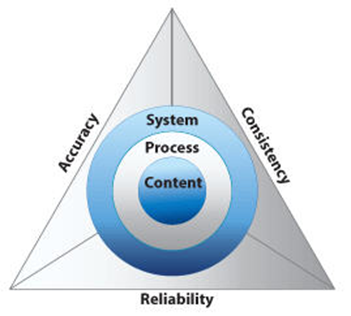
\includegraphics[width=3in]{toanvendulieu}
\caption[Toàn ven dữ liệu]{Toàn ven dữ liệu}
\label{fig:toanvendulieu}
\end{figure}
\end{center}

\subsubsection*{Đồng bộ hóa} Hệ thống giám sát môi trường có nhiều thiết thiết bị khác nhau, nhiều phương pháp và cách thức truyền dữ liệu khác nhau. Do đó ta cần phải có sự chuẩn hóa các giao thức giao tiếp, đồng bộ các gói dữ liệu. Tuy nhiên điều này sẽ dẫn đến vấn nạn được đề cập ở mục sau.

\subsubsection*{Tính bảo mật} Vấn đề bảo mật và an toàn dữ liệu hiện tại vẫn là một trong những khó khăn mà hệ thống IoT đang mắc phải. Vì hệ thống IoT đòi hỏi cần phải có giao thức kết nối giữa các thiết bị phải được chuẩn hóa và động bộ, cũng như tối giản kích thước gói tin để tối ưu trong việc truyền dữ liệu giữa các thiết bị, do đó gói tin truyền đi có thiết lập cấu trúc đơn giản và hệ thống dễ bị thâm nhập. Điều này sẽ dẫn đến hệ thống có thể bị đánh cắp dữ liệu, và thậm chí mất quyền kiểm soát toàn bộ hệ thống bởi vì tất cả đều được kết nối với nhau. Vậy nên cần phải cân nhắc trade-off giữa hiệu năng hệ thống và tính bảo mật.
\begin{figure}[H]
\centering    
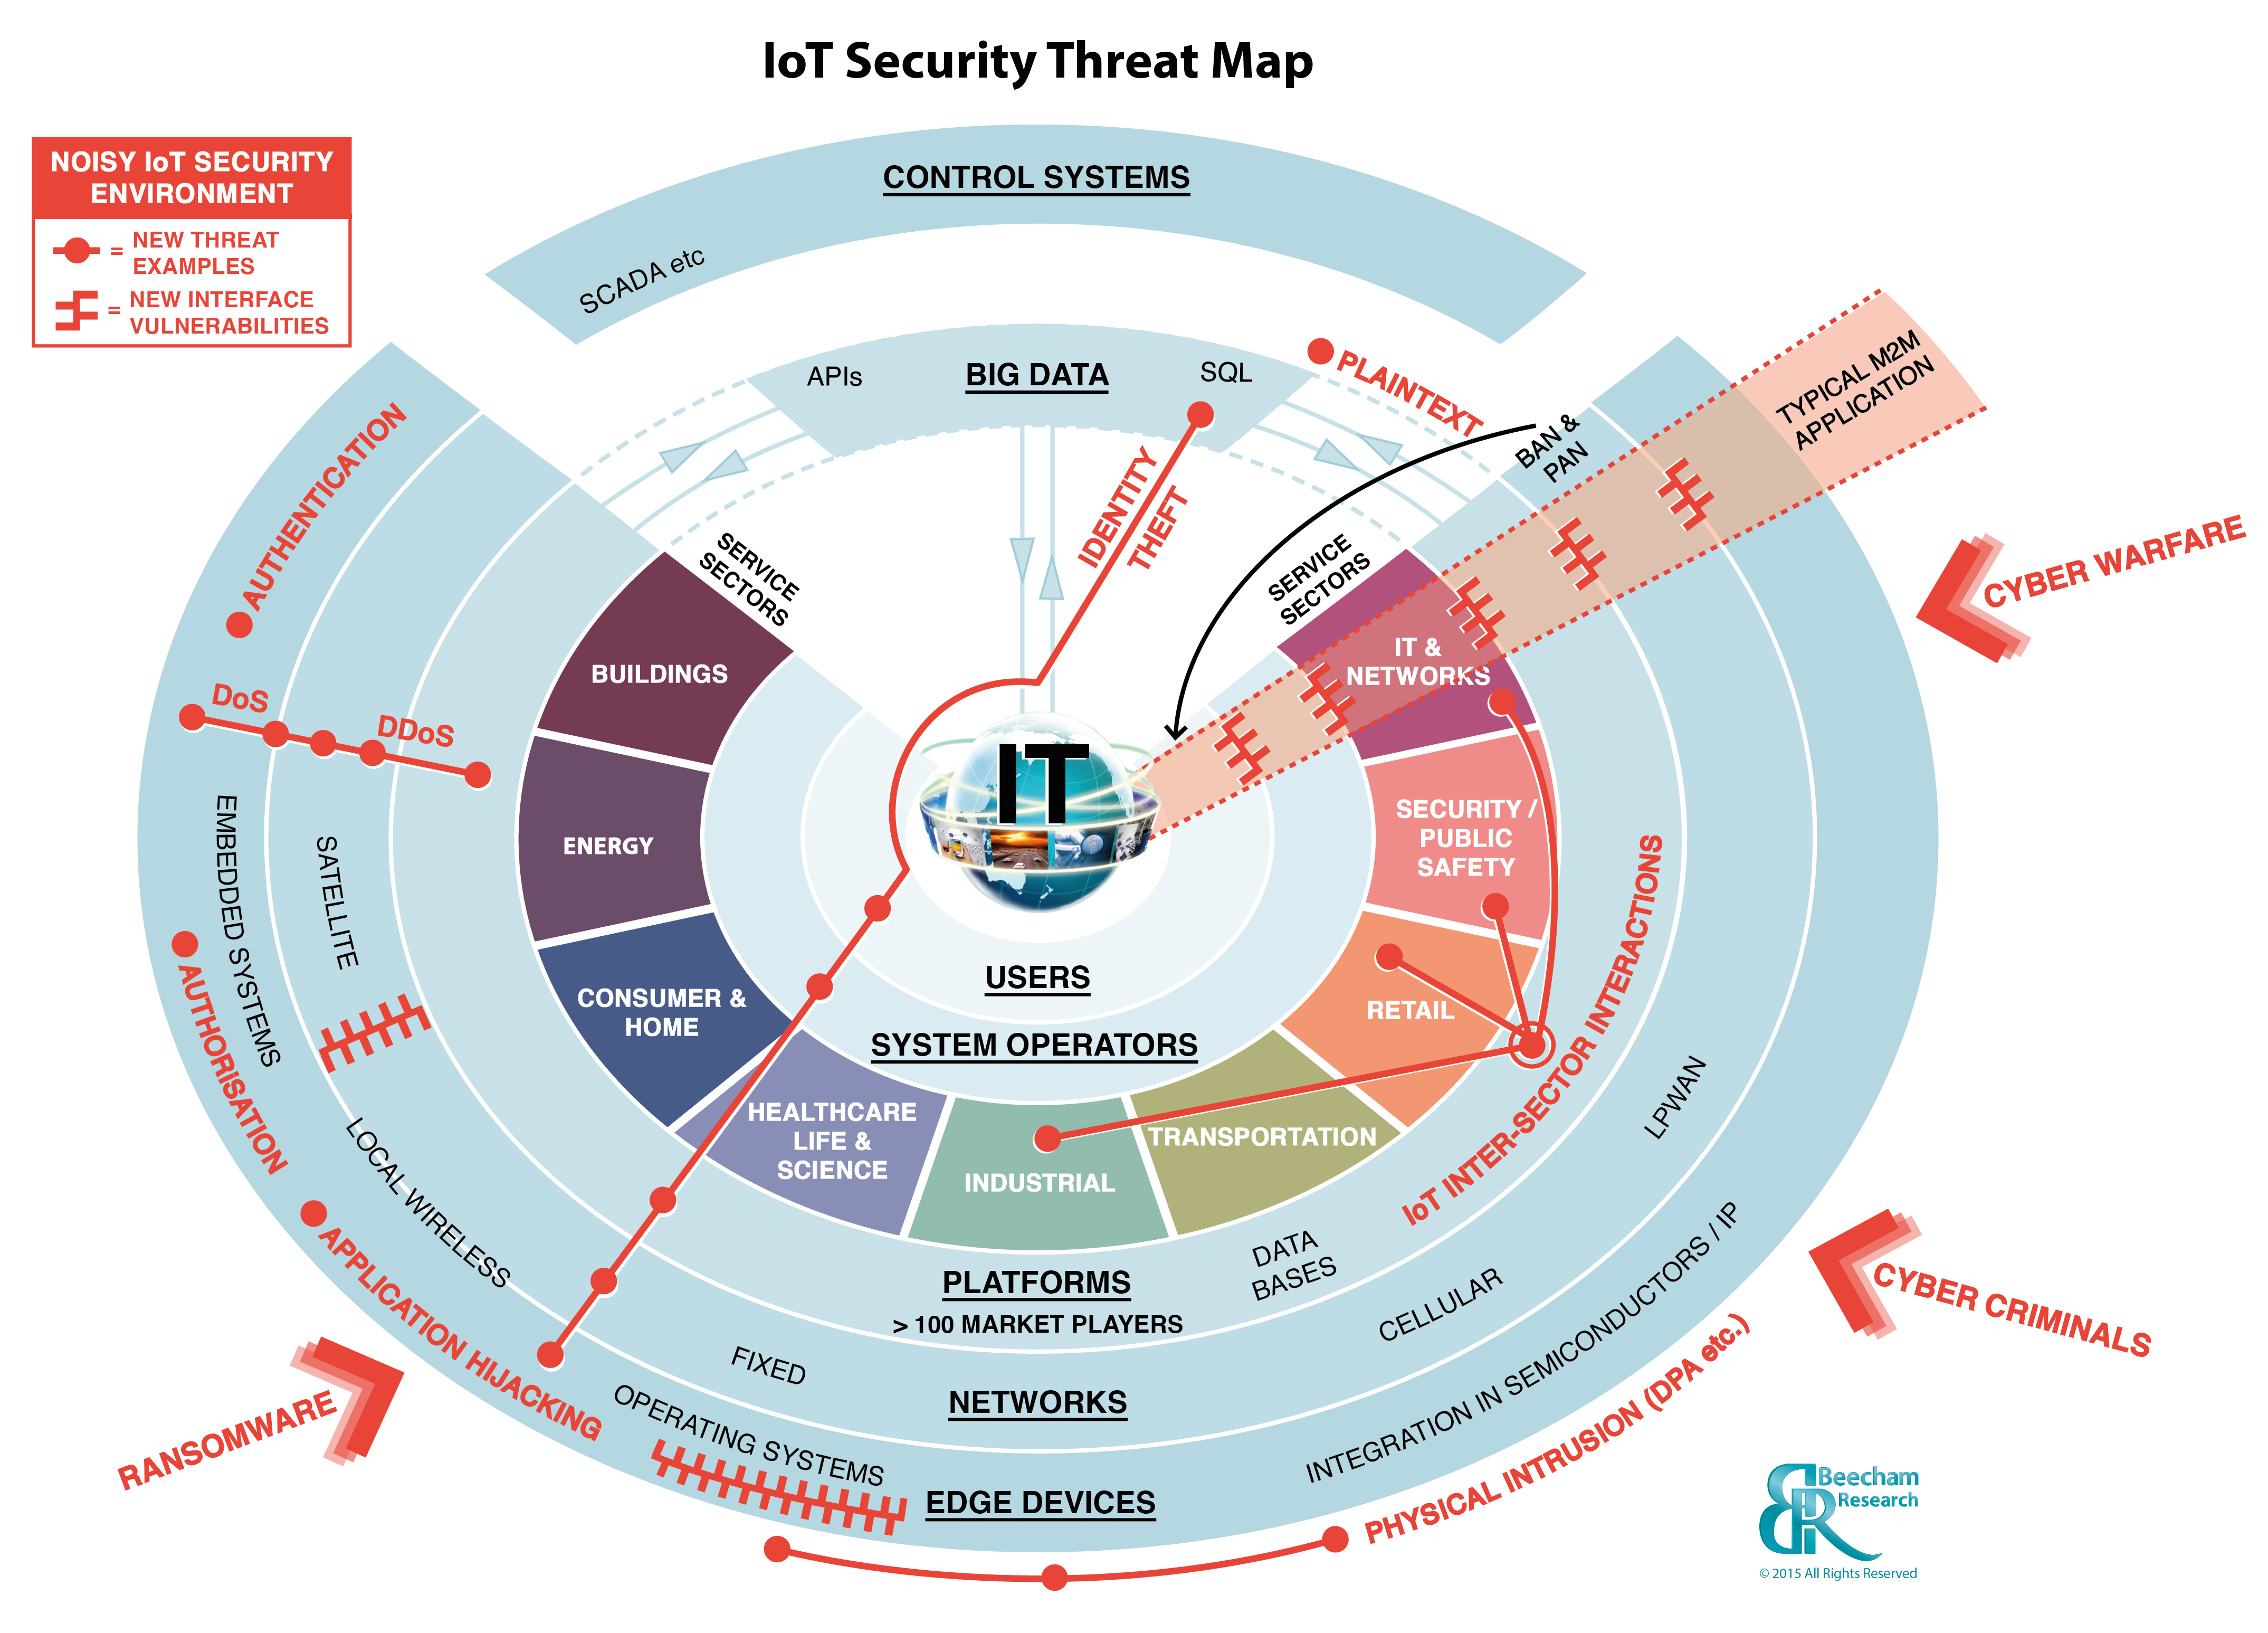
\includegraphics[width=5in]{virusiot}
\caption[Tính bảo mật]{Tính bảo mật}
\label{fig:virusiot}
\end{figure}

Các mối nguy hại chính ảnh hưởng trực tiếp tới hệ thống IoT như: DDoS, Ransomware, Cyber Criminals và Cyber Warfare. 



\newpage

\section{Hiện thực node cảm biến}
\subsection{Hiện thực prototype node cảm biến}
Chức năng chính của node cảm biến là dùng để lấy các dữ liệu môi trường như giá trị nồng độ CO, chất lượng không khí, nhiệt độ và lượng bụi, trong quá trình tìm các loại cảm biến trên thị trường hiện có thì nhóm chúng tôi đã đề xuất sử dụng các cảm biến được đề cập tại mục \ref{sec:cacloaicambien} như sau:
\begin{itemize}
\item[•]Cảm biến GP2: dùng để đo lượng bụi có trong không khí.
\item[•]Cảm  biến MQ135: dùng để đo chất lượng của môi trường không khí.
\item[•]Cảm biến MQ07: dùng để đo nồng độ khí CO trong không khí.
\item[•]Cảm biến DS18B20: dùng để đo nhiệt độ môi trường xung quanh. 
\end{itemize}
Như vậy, các thành phần chính của prototype biến đầu tiên chúng tôi đã xây dựng như sau:
\begin{figure}[H]
\centering    
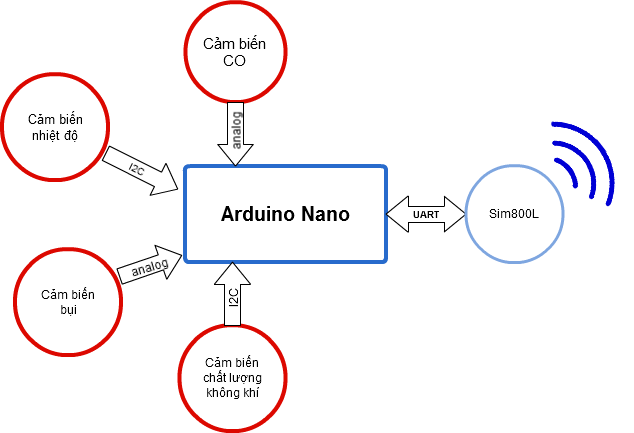
\includegraphics[width=5in]{prototype_1}
\caption[Mô hình prototype đầu tiên]{Mô hình prototype đầu tiên}
\label{fig:prototype_1}
\end{figure}
Ngoài những cảm biến đã đề cập thì sơ đồ hoạt động của các khối chức năng trong Hình \ref{fig:prototype_1} còn có thêm những khối chính sau:
\begin{itemize}
\item[•] Khối Arduino Nano: mạch xử lý trung tâm có nhiệm vụ định thời và điều khiển các khối cảm biến khác để thu thập dữ liệu cảm biến sau đó sẽ xử lý các số liệu thô sang số liệu chính xác, cuối cùng gửi dữ liệu đã được xử lý lên cho máy chủ thông qua khối Sim800L.
\item[•] Khối Sim800L: chức năng mở kết nối TCP tới máy chủ thông qua dịch vụ GPRS của nhà mạng cung cấp và đưa các dữ liệu từ mạch vi xử lý gửi thông qua giao thức UART.
\end{itemize}



\subsubsection*{Mô hình khối nguồn cho node cảm biến}
Tiếp đến phần thiết kế thì để có thể tận dụng nguồn năng lượng mặt trời để nạp pin cho mạch hoạt động độc lập với điện lưới thì chúng tôi đã đề xuất mô hình khối nguồn như sau:
\begin{figure}[H]
\centering    
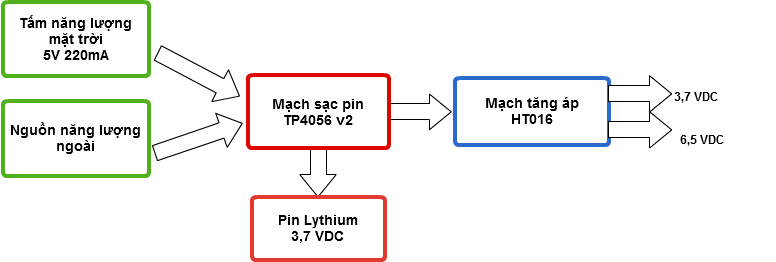
\includegraphics[width=6in]{khoinguon}
\caption[Mô hình khối nguồn]{Mô hình khối nguồn}
\label{fig:khoinguon}
\end{figure}

\begin{itemize}
\item[•]Mạch tăng áp mini HT106 là module tăng áp cực kì nhỏ gọn, ngõ vào là cổng mircoUSB. Mạch có khả năng tăng đến 28v tối đa. Dưới đây là một số thông số kỹ thuật:\\
-	Điện áp vào: 2-24V\\
-	Điện áp ra: 5-28V\\
-	Dòng tối đa: 2A đỉnh, dòng liên tục khoảng 1A.\\
-	Công suất: 6W\\
-	Hiệu suất: 93%
	\begin{figure}[H]
	\centering    
	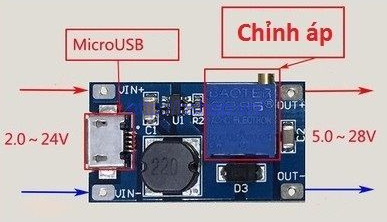
\includegraphics[width=3in]{ht06}
	\caption[Mạch tăng áp mini HT106]{Mạch tăng áp mini HT106}
	\label{fig:ht06}
	\end{figure}

\item[•]Mạch sạc pin Lithium TP4056v2 sử dụng IC quản lý sạc TP4056 nhưng được nâng cấp để có thể ngắt khi pin yếu dưới 2.4V nhằm bảo vệ pin. Một số thông số kỹ thuật của mạch sạc pin Lithium TP4056v2\\
-	Điện áp đầu vào: 5VDC mini USB\\
-	Điện áp ngưỡng ra tự động ngắt: 4.2V +- 1%\\
-	Dòng sạc tối đa: 1000mA\\
-	Điện áp ngưỡng cần sạc là 2.5V\\
-	Tích hợp tự động ngắt bảo vệ pin khi pin yếu dưới 2.4 V qua 2 chân OUT+ và OUT-
	\begin{figure}[H]
	\centering    
	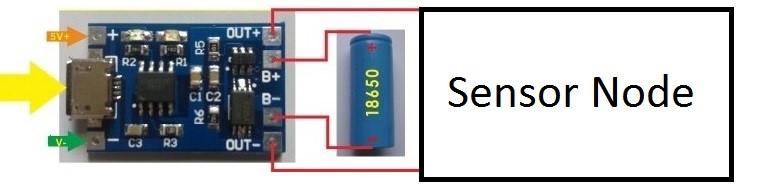
\includegraphics[width=5in]{tp4056}
	\caption[Mạch sạc pin Lithium TP4056v2]{Mạch sạc pin Lithium TP4056v2}
	\label{fig:tp4056}
	\end{figure}
\item[•]Pin năng lượng mặt trời Poly 5.5V /220 mA\\
-	Với kích thước: 100x80x2mm\\
-	Nguồn đầu ra: 5.5V\\
-	Dòng tối đa cung cấp được: 220mA\\
\begin{figure}[H]
\centering    
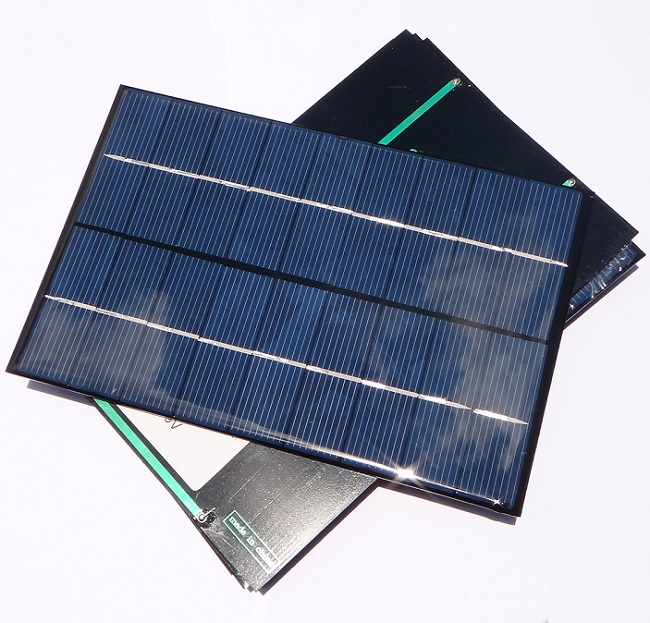
\includegraphics[width=0.6\textwidth]{solarpanel_real}
\caption[Pin năng lượng mặt trời Poly 5V /220 mA]{Pin năng lượng mặt trời Poly 5V /220 mA}
\label{fig:solarpanel_real}
\end{figure}

\item[•]Nguồn năng lượng ngoài: sử dụng trong một số trường hợp thời tiết mưa nhiều hoặc gió nhiều mà thiếu nguồn năng lượng mặt trời, chúng ta có thể tận dụng nguồn mưa và gió nhờ các tuapin phát năng lượng nhờ vào sức gió và mưa.
\item[•] Nguồn đầu ra 3.7VDC dùng để cấp cho module Sim800L còn đối với nguồn 6.5VDC dùng để cung cấp cho mạch vi xử lý.
\end{itemize}





\subsubsection*{Các thư viện đã sử dụng} 
\begin{lstlisting}[language=C]
#include "MQ135.h" //Thu vien cac ham toan hoc de xu ly so lieu MQ135
#include "MQ07.h" //Thu vien cac ham toan hoc de xu ly so lieu MQ07
#include "OneWire.h" // Thu vien cau hinh giao thuc I2C
#include "DallasTemperature.h" // Thu vien cho cam bien nhiet do
#include "SoftwareSerial.h" // Thu vien mo rong cac chan UART
#include "TimerOne.h" // Thu vien cau hinh timer
\end{lstlisting}



\subsubsection*{Kết quả hiện thực}
\begin{figure}[H]
\centering    
\includegraphics[width=5in]{prototype_2}
\caption[Kết quả prototype đầu tiên]{Kết quả prototype đầu tiên}
\label{fig:prototype_2}
\end{figure}

\begin{figure}[H]
\centering    
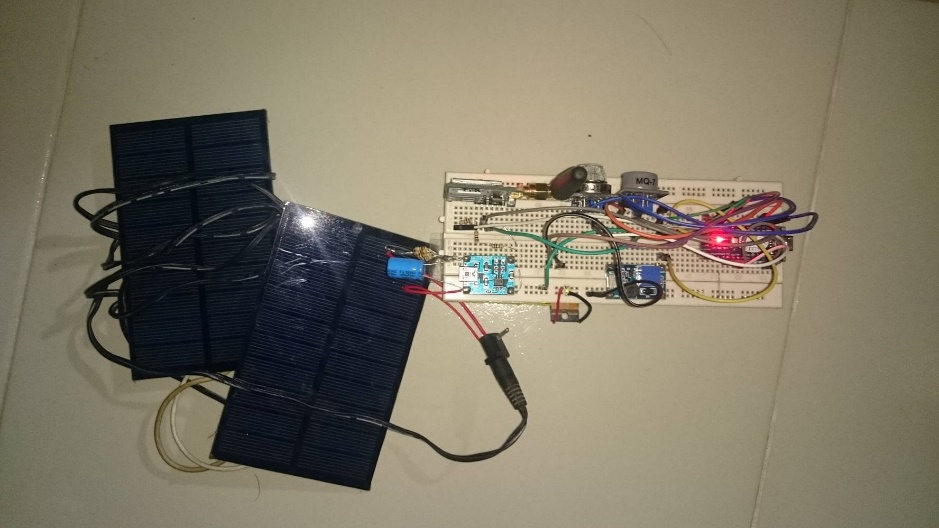
\includegraphics[width=5in]{prototype_3}
\caption[Kết quả prototype đầu tiên 2]{Kết quả prototype đầu tiên 2}
\label{fig:prototype_3}
\end{figure}



\subsubsection*{Nhận xét}
\begin{itemize}
\item[•] Hoàn thành các chức năng có thể đọc được các dữ liệu từ cảm biến MQ135, MQ07, DS18B20, và GP2.
\item[•] Xử lý được dữ liệu thông qua các thư viện do nhà sản xuất cảm biến cung cấp.
\item[•] Gửi được dữ liệu lên máy chủ thông qua dịch vụ GPRS của Sim800L, hệ thống máy chủ của chúng tôi ban đầu chưa được hoàn thành nên nhờ đến công cụ phát triển IoT Thingspeak thì chúng tôi đã kiểm tra được, xem thêm tại: \url{https://thingspeak.com/channels/157120}
\end{itemize}




\subsection{Hiện thực mô hình tổng thể node cảm biến}
\subsubsection*{Hoàn thiện chức năng}
Sau khi hoàn thành prototype đầu tiên node cảm biến thì chúng tôi đã bắt đầu lên kế hoạch nâng cấp chúng thêm những chức năng để có thể tối ưu tốt nhất có thể. Chức năng của node cảm biến bao gồm:
\begin{itemize}
\item[•] 
\item[•]
\item[•]
\end{itemize}

\subsubsection*{Hiện thực board mạch vi xử lý}
Board mạch vi xử lý được thiết kế và hiện thực gọn nhất có thể và hỗ trợ các header nối các dây bus đến các cảm biến và module Sim800L. Chúng tôi đã thực hiện thiết kế board mạch vi xử lý như Hình \ref{fig:botrimcu}

\begin{figure}[H]
\centering  
  \begin{subfigure}[b]{0.5\textwidth}
    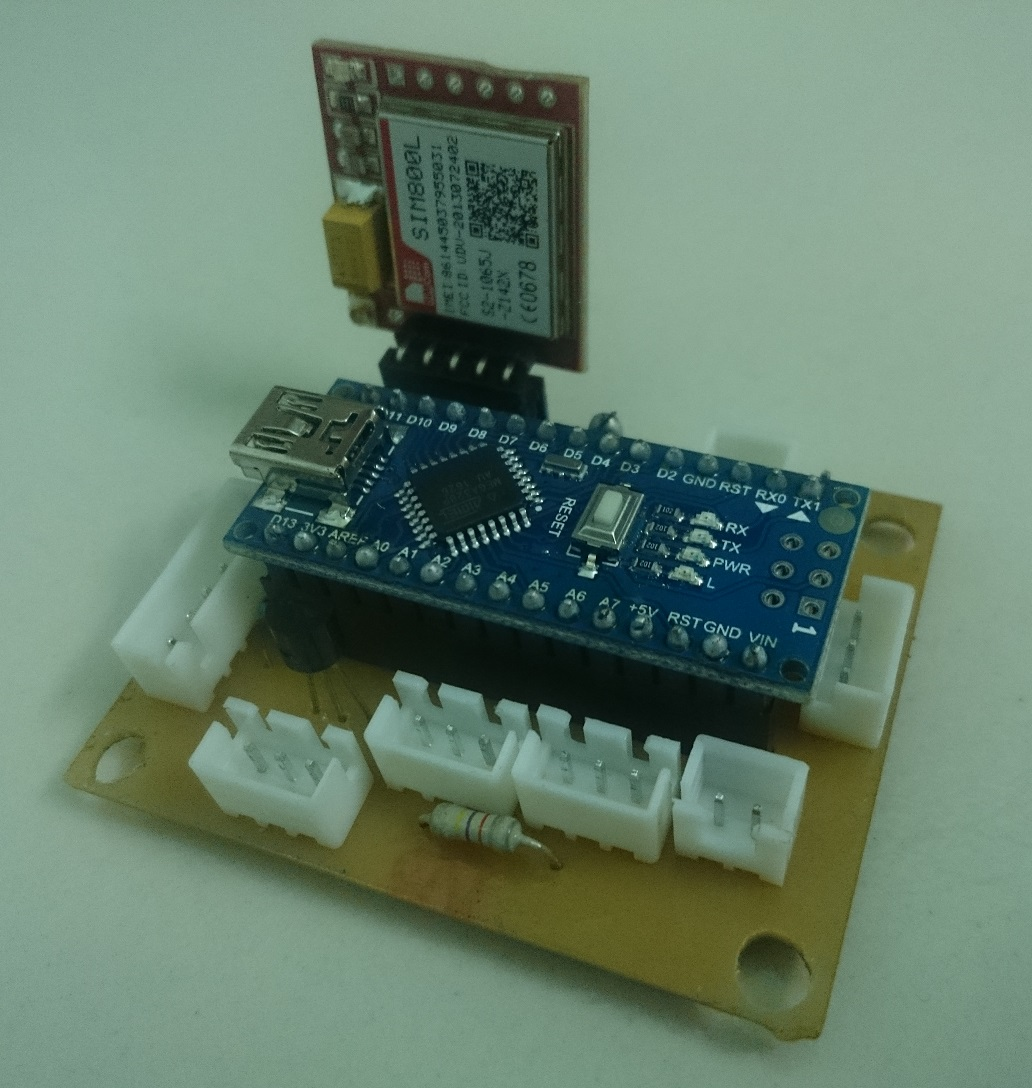
\includegraphics[width=3in]{mcu}
    \caption[Mô hình 1]{Mô hình 1}
    \label{fig:mcu}
  \end{subfigure}\hfill
  \begin{subfigure}[b]{0.5\textwidth}
    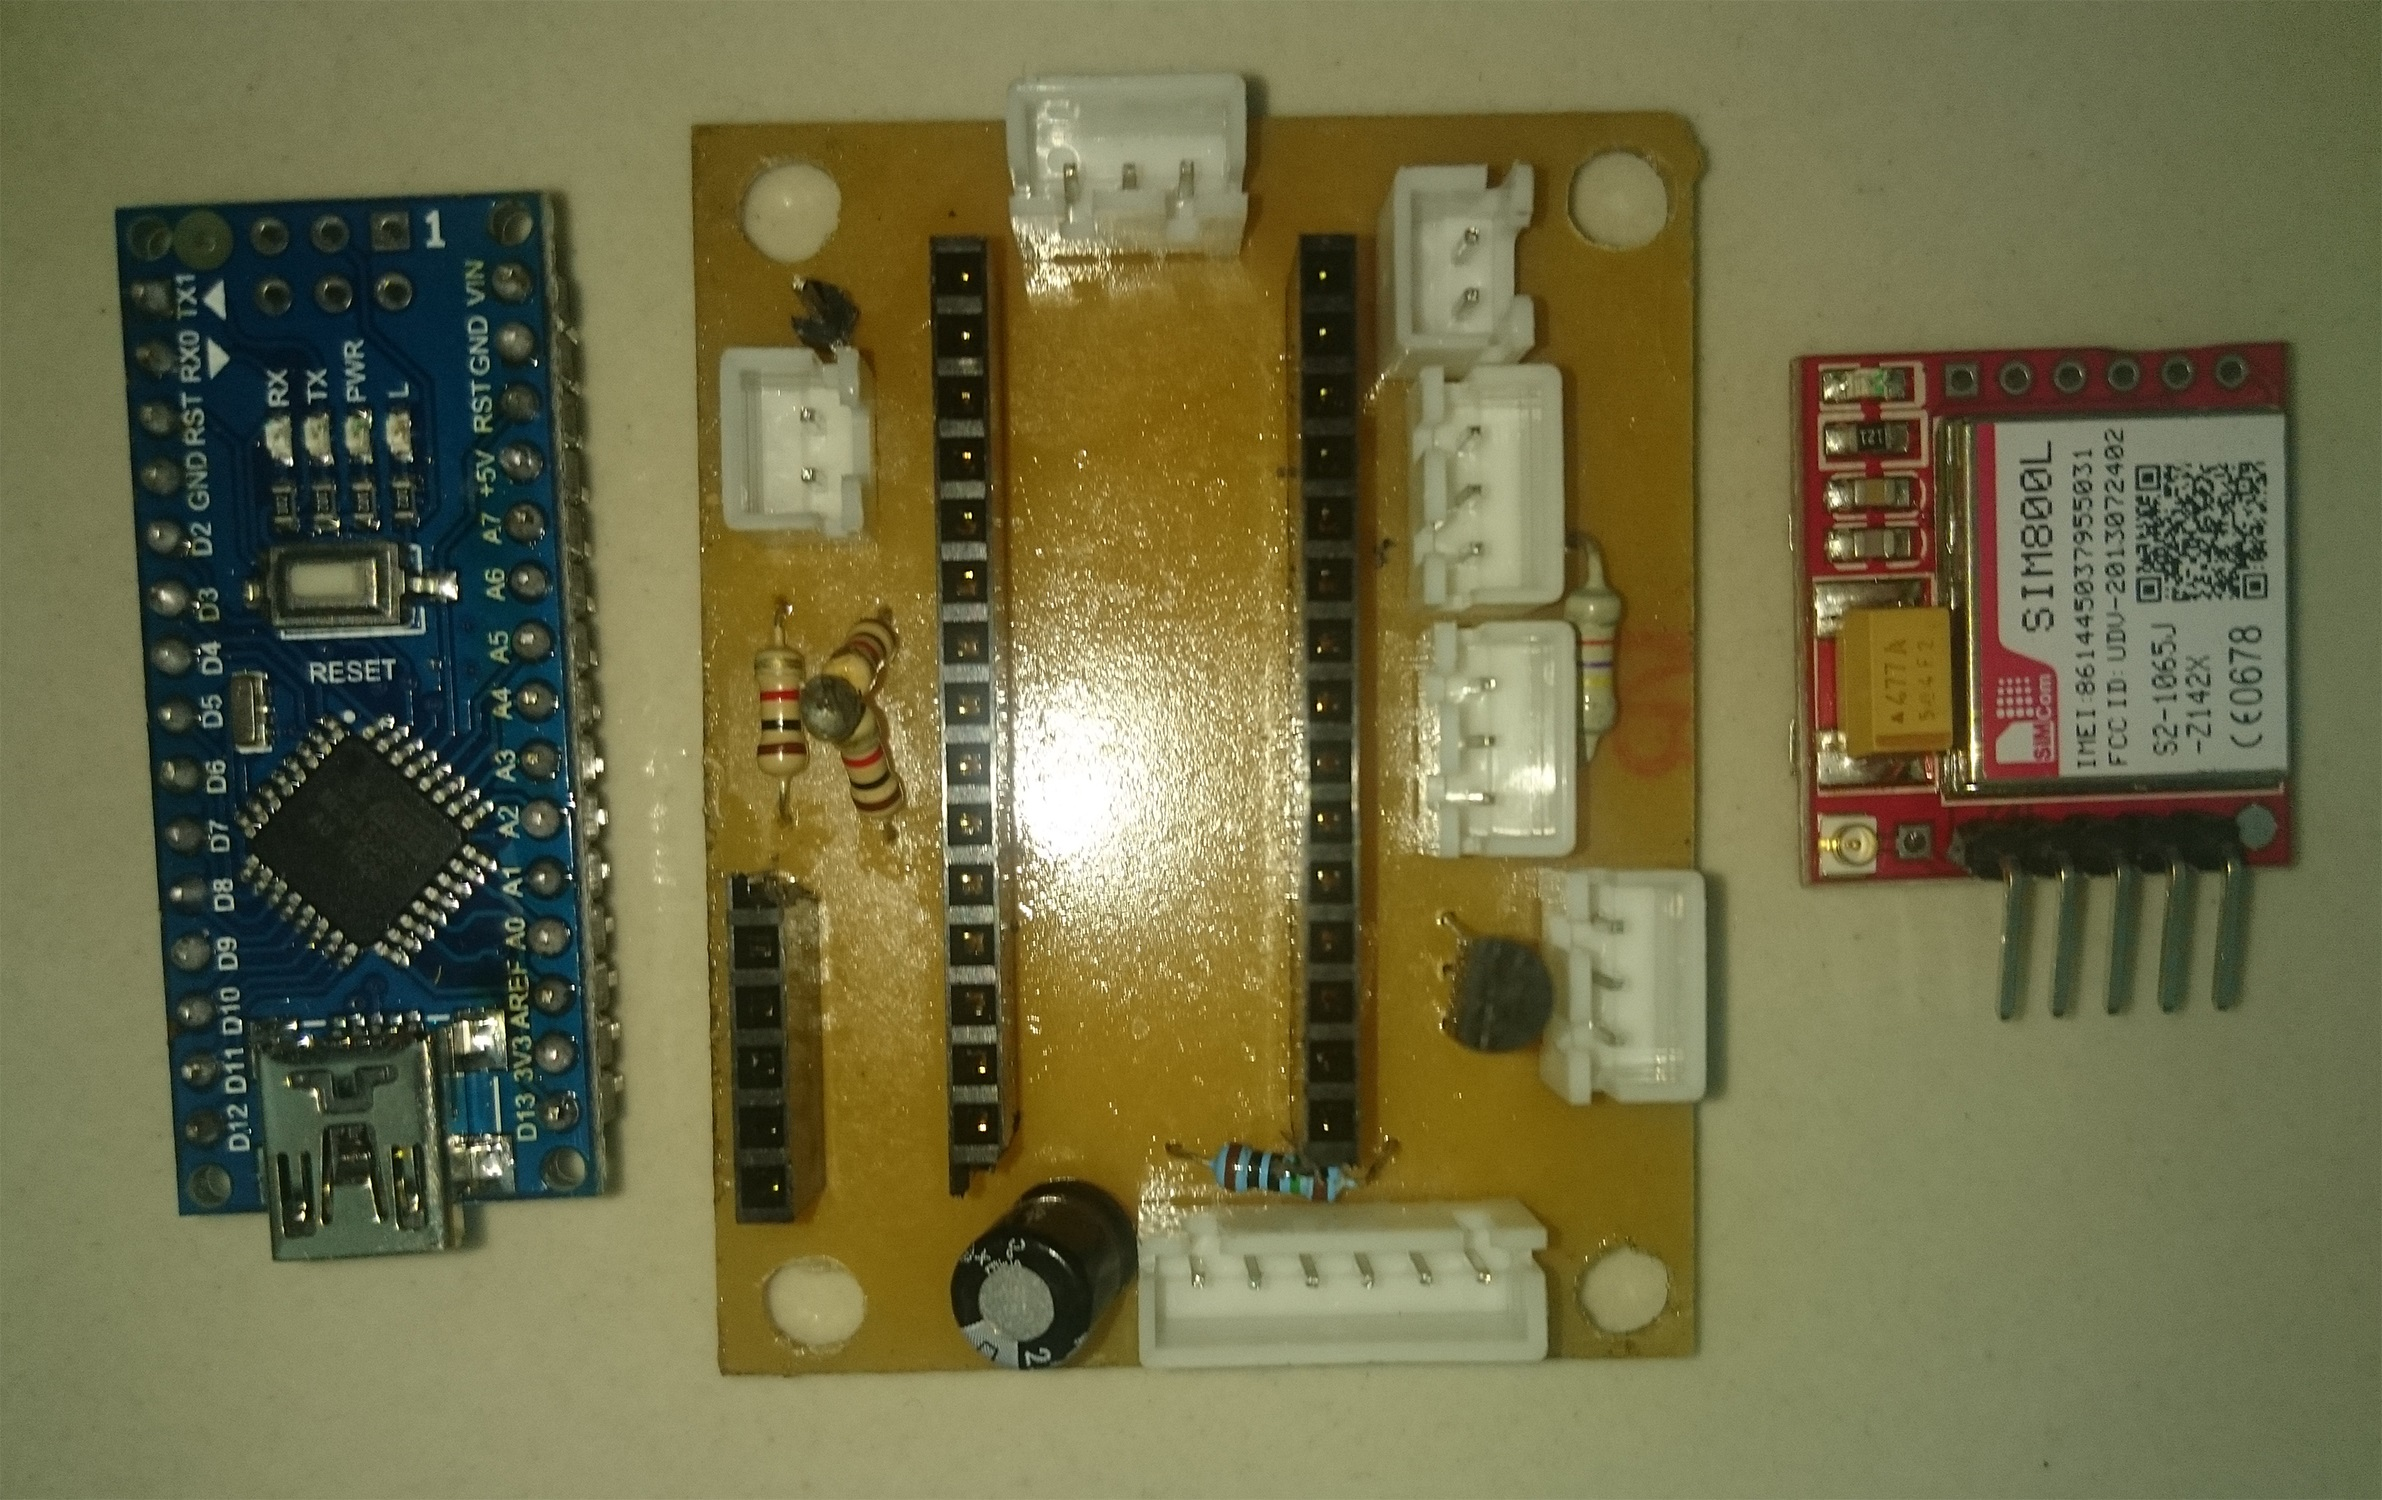
\includegraphics[width=3in]{mcu_2}
  	 \caption[Mô hình 2]{Mô hình 2}
    \label{fig:mcu_2}
  \end{subfigure}
  \caption{Bố trí board mạch vi xử lý}\label{fig:botrimcu}
\end{figure}

Một số khai báo được sử dụng như sau:
\begin{lstlisting}[numbers=left,firstnumber=1,language=C]
#define ONE_WIRE_BUS 4
#define MQ135_PIN A0
#define MQ7_PIN A1
#define RX_SIM_OUT 11
#define TX_SIM_OUT 10
#define DUST_OUT A2
#define DUST_PIN 2

// Gia tri % Pin thap se khong cho phep mach hoat dong
#define LOW_BATTERY 30 

// So lan gui lai du lieu len may chu neu khong thanh cong
#define TIMEFAIL_SENDSMS 5 

// Mo rong UART tren chan so 11 va 10
SoftwareSerial sim900(RX_SIM_OUT, TX_SIM_OUT);

int TIMEON = 3; //Thoi gian dot nong cam bien MQ135, MQ07

//Thoi gian ngat nguon cam bien MQ135, MQ07 ban ngay
int TIMEOFF_DAY = 13; 
//Thoi gian ngat nguon cam bien MQ135, MQ07 ban dem
int TIMEOFF_NIGHT = 28;

// Moc thoi gian xac dinh buoi sang va buoi toi
int time_s1 = 6;
int time_s2 = 19;

String apiKey = "7"; //Node ID
\end{lstlisting}
Lập trình cho vi xử lý Arduino Nano được mô hình hóa theo lưu đồ xử lý dưới Hình \ref{fig:node_status}:

\begin{figure}[H]
\centering    
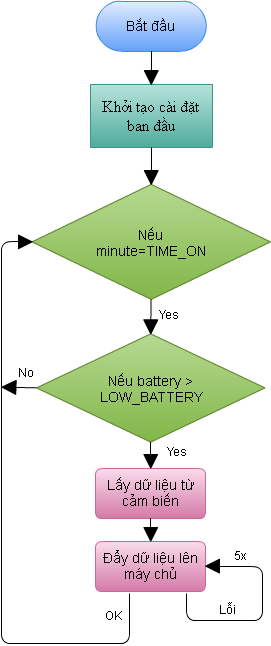
\includegraphics[width=2.5in]{node_status}
\caption[Lưu đồ xử lý hàm main]{Lưu đồ xử lý hàm main}
\label{fig:node_status}
\end{figure}

\begin{itemize}
\item[•]Khởi tạo cài đặt ban đầu gồm các công việc: \\
- Thiết lập chế độ hoạt động của các chân trên vi xử lý.\\
- Thiết lập tốc độ truyền UART.\\
- Thiết lập timer định thời.\\
- Khởi động Module Sim800L.\\
- Đồng bộ thời gian module Sim800L với máy chủ The Network Time Protocol(NTP).\\

Việc Đồng bộ thời gian module Sim800L với máy chủ NTP được Sim800L hỗ trợ qua các tập lệnh sau:
\begin{lstlisting}[numbers=left,firstnumber=1,language=C]
void syncTime()
{
  //  Network time sync
  sim900.println("AT+SAPBR=1,1");
  delay(2000);
  sim900.println("AT+CNTPCID=1");
  delay(2000);
  sim900.println("AT+CNTP=\"128.4.24.98\",28");
  delay(2000);
  sim900.println("AT+CNTP");
  delay(4000);  
  sim900.println("AT+SAPBR=0,1");
  delay(2000);
  Serial.println("Sync time - Done");
  updateTime();
}
\end{lstlisting}







\end{itemize}









\subsubsection*{Bố trí các linh kiện trong hộp cảm biến}
Việc bố trí các linh kiện trong hộp cảm biến nhầm giúp cho việc thu thập dữ liệu của các cảm biến được hiệu quả hơn và không bị ảnh hưởng bởi mưa. Nó cũng giúp cho việc phát triển trong tương lai nếu các cảm biến hoặc linh kiện bị hư thì dễ dàng thay thế hơn.

Đối với các cảm biến MQ135, MQ07 và cảm biến nhiệt DS18B20 thì được bố trí đặt ở lớp dưới của chiếc hộp như Hình \ref{fig:botri}

\begin{figure}[H]
\centering  
  \begin{subfigure}[b]{0.5\textwidth}
    
\includegraphics[width=2.5in]{house_sensor}
    \caption[Mô hình]{Mô hình}
    \label{fig:house_sensor}
  \end{subfigure}\hfill
  \begin{subfigure}[b]{0.5\textwidth}
    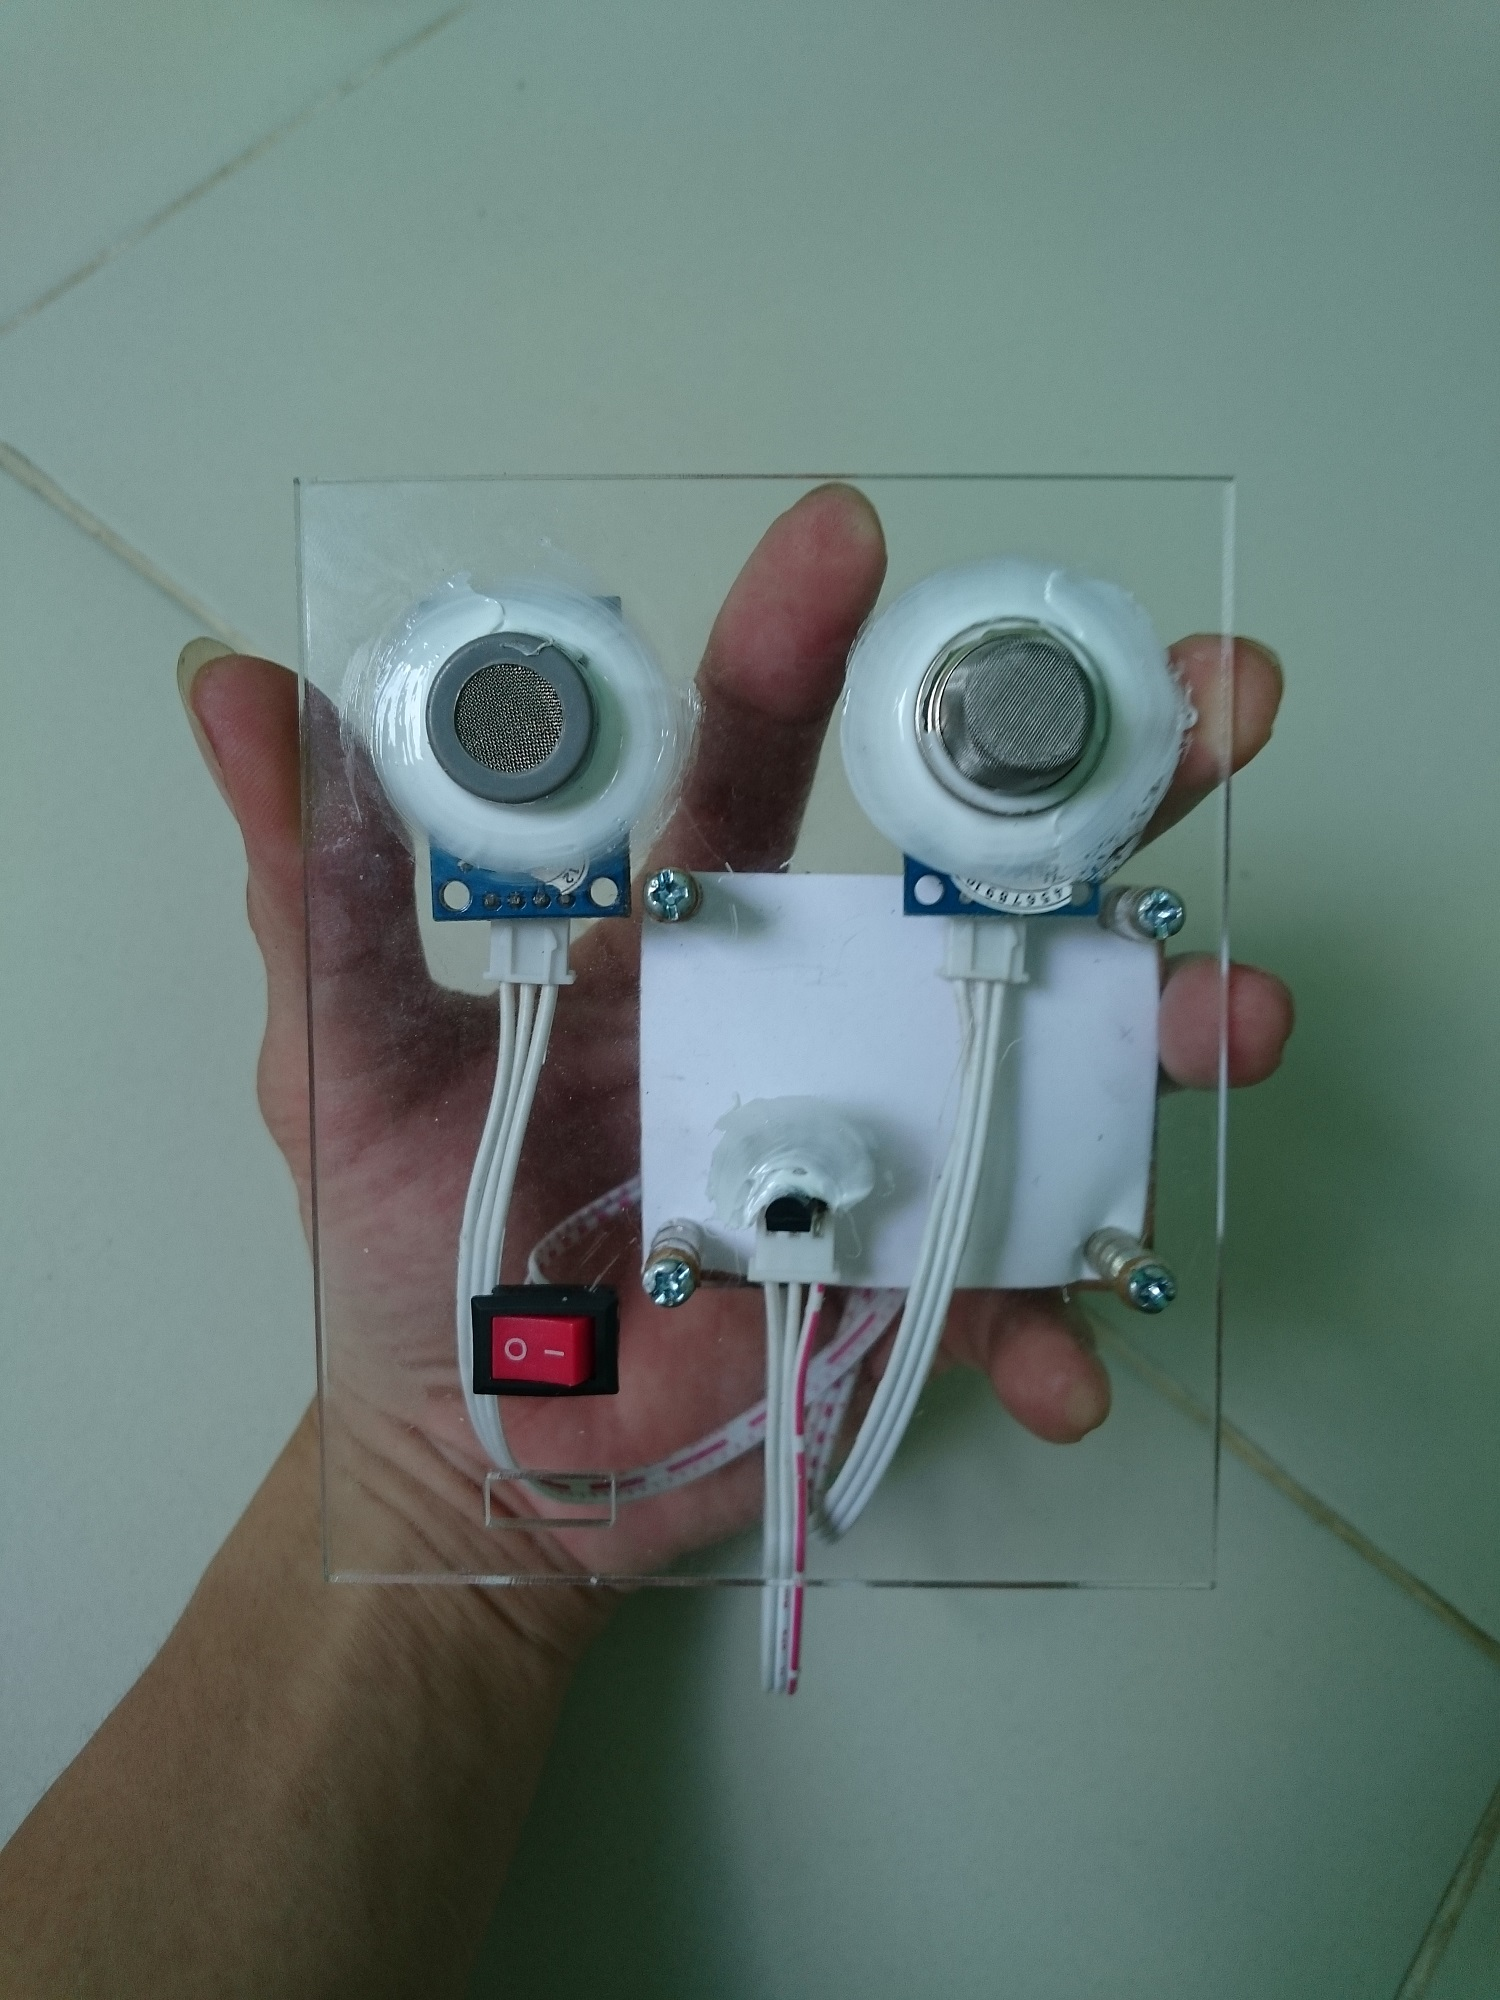
\includegraphics[width=2.5in]{house_sensor_2}
  	 \caption[Thực tế]{Thực tế}
    \label{fig:house_sensor_2}
  \end{subfigure}
  \caption{Bố trí các cảm biến}\label{fig:botri}
\end{figure}
Đối với các cảm biến bụi GP2 chúng tôi đề xuất vị trí được đặt như Hình \ref{house_dust} sau:
\begin{figure}[H]
\centering    
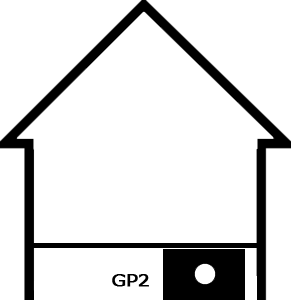
\includegraphics[width=2.5in]{house_dust}
\caption[Mô hình đặt cảm biến GP2]{Mô hình đặt cảm biến GP2}
\label{fig:house_dust}
\end{figure}
Còn các board mạch vi xử lý, module Sim800L và pin được đặc vị trí bên trong chiếc hộp như Hình \ref{fig:house_board_kogps} sau:
\begin{figure}[H]
\centering    
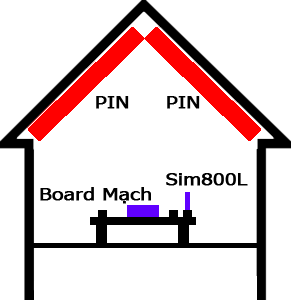
\includegraphics[width=2.5in]{house_board_kogps}
\caption[Mô hình bố trị các linh kiện khác]{Mô hình bố trị các linh kiện khác}
\label{fig:house_board_kogps}
\end{figure}



\newpage
\subsection{Mức độ tiêu hao năng lượng}
Để biết được mức tiêu hao năng lượng của mạch hoạt động như thế nào thì chúng tôi đã bắt đầu tính toán từ những thông số tiêu thụ chuẩn của các linh kiện được sử dụng trong node cảm biến. Nhầm nắm bắt được và đưa ra dung lượng pin cần thiết cho các node cảm biến chạy mà không phụ thuộc vào mạng lưới điện.\\
Chú ý: các thông số tính toán dưới lấy từ thông số chuẩn của nhà sản xuất kèm với một số thông số chuẩn của chúng tôi như sau:
\begin{itemize}
\item[•] Thời gian cho việc đốt nóng cảm biến MQ135 và MQ07 trước khi lấy dữ liệu: 3 phút
\item[•] Ban ngày từ 7AM-8PM: cứ mỗi 15 phút gửi dữ liệu lên máy chủ.
\item[•] Ban đêm từ 8PM-7AM: cứ mỗi 30 phút gửi dữ liệu lên máy chủ.
\end{itemize}

Mức tiêu hao năng lượng vào 1 buổi sáng 7AM-8PM:

\begin{table}[H]
\centering
\caption{Bảng tiêu thụ năng lượng buổi sáng}
\label{table:buoisang}
\begin{tabular}{|l|l|r|r|r|r|}
\hline
\textbf{STT}  & \textbf{Module}                                                       & \multicolumn{1}{c|}{\textbf{\begin{tabular}[c]{@{}c@{}}Dòng tiêu \\ thụ (mA)\end{tabular}}} & \multicolumn{1}{c|}{\textbf{\begin{tabular}[c]{@{}c@{}}Giờ hoạt \\ động (h)\end{tabular}}} & \multicolumn{1}{c|}{\textbf{\begin{tabular}[c]{@{}c@{}}Tổng dòng \\ tiêu thụ(mA)\end{tabular}}} & \multicolumn{1}{c|}{\textbf{\begin{tabular}[c]{@{}c@{}}Công suất\\ (mW)\end{tabular}}} \\ \hline
1             & Cảm biến bụi                                                          & 20                                                                                          & 13                                                                                         & 260                                                                                             & 858                                                                                    \\ \hline
2             & Cảm biến MQ07                                                         & 250                                                                                         & 2.6                                                                                        & 650                                                                                             & 3250                                                                                   \\ \hline
3             & Cảm biến MQ135                                                        & 300                                                                                         & 2.6                                                                                        & 780                                                                                             & 3900                                                                                   \\ \hline
4             & \begin{tabular}[c]{@{}l@{}}Cảm biến nhiệt độ\\ 18BS20\end{tabular}    & 1.5                                                                                         & 13                                                                                         & 19.5                                                                                            & 97.5                                                                                   \\ \hline
5             & \begin{tabular}[c]{@{}l@{}}Module Sim800L \\ (idea mode)\end{tabular} & 10                                                                                          & 12.35                                                                                      & 123.5                                                                                           & 456.95                                                                                 \\ \hline
6             & \begin{tabular}[c]{@{}l@{}}Module Sim800L\\ (Hoạt động)\end{tabular}  & 500                                                                                         & 0.65                                                                                       & 325                                                                                             & 1202.5                                                                                 \\ \hline
7             & Arduino nano                                                          & 10                                                                                          & 13                                                                                         & 130                                                                                             & 780                                                                                    \\ \hline
\textbf{Tổng} & \textbf{}                                                             & \textbf{1091.5}                                                                             & \textbf{}                                                                                  & \textbf{2288}                                                                                   & \textbf{10544.95}                                                                      \\ \hline
\end{tabular}
\end{table}


Mức tiêu hao năng lượng vào 1 buổi tối 8PM-7AM:
\begin{table}[H]
\centering
\caption{Bảng tiêu thụ năng lượng buổi tối}
\label{table:buoitoi}
\begin{tabular}{|l|l|r|r|r|r|}
\hline
\textbf{STT}  & \textbf{Module}                                                       & \multicolumn{1}{c|}{\textbf{\begin{tabular}[c]{@{}c@{}}Dòng tiêu \\ thụ (mA)\end{tabular}}} & \multicolumn{1}{c|}{\textbf{\begin{tabular}[c]{@{}c@{}}Giờ hoạt \\ động (h)\end{tabular}}} & \multicolumn{1}{c|}{\textbf{\begin{tabular}[c]{@{}c@{}}Tổng dòng \\ tiêu thụ(mA)\end{tabular}}} & \multicolumn{1}{c|}{\textbf{\begin{tabular}[c]{@{}c@{}}Công suất\\ (mW)\end{tabular}}} \\ \hline
1             & Cảm biến bụi                                                          & 20                                                                                          & 11                                                                                         & 220                                                                                             & 726                                                                                    \\ \hline
2             & Cảm biến MQ07                                                         & 250                                                                                         & 2.2                                                                                        & 550                                                                                             & 2750                                                                                   \\ \hline
3             & Cảm biến MQ135                                                        & 300                                                                                         & 2.2                                                                                        & 660                                                                                             & 3300                                                                                   \\ \hline
4             & \begin{tabular}[c]{@{}l@{}}Cảm biến nhiệt độ\\ 18BS20\end{tabular}    & 1.5                                                                                         & 11                                                                                         & 16.5                                                                                            & 82.5                                                                                   \\ \hline
5             & \begin{tabular}[c]{@{}l@{}}Module Sim800L \\ (idea mode)\end{tabular} & 10                                                                                          & 10.45                                                                                      & 104.5                                                                                           & 386.65                                                                                 \\ \hline
6             & \begin{tabular}[c]{@{}l@{}}Module Sim800L\\ (Hoạt động)\end{tabular}  & 500                                                                                         & 0.55                                                                                       & 275                                                                                             & 1017.5                                                                                 \\ \hline
7             & Arduino nano                                                          & 10                                                                                          & 11                                                                                         & 110                                                                                             & 660                                                                                    \\ \hline
\textbf{Tổng} & \textbf{}                                                             & \textbf{1091.5}                                                                             & \textbf{}                                                                                  & \textbf{1936}                                                                                   & \textbf{8922.65}                                                                       \\ \hline
\end{tabular}
\end{table}

\section{Hệ thống Server lưu trữ dữ liệu và cung cấp API}

\subsection{Cấu trúc tổ chức tập tin}
\subsubsection*{Các thư mục và chức năng}
Chúng ta có những thư mục được làm việc trực tiếp:

• libs: chứa các hàm function hỗ trợ về xác thực và log.

• models: thư mục này bao gồm các mô hình quản lý cơ sở dữ liệu.

• routes: điều khiển và điều hướng theo các url.

• log: chứa các file ghi lại log trong quá trình hoạt động.

• views: là bộ mặt của web server, giúp người dùng có thể tương tác được với server qua web browser, bao gồm các file giao diện như html, ejs...   


\subsubsection*{Các file khởi tạo và cấu hình Server}

\textbf{Các file khởi tạo này bao gồm:}

• emap.js: file có chức năng đọc file cấu hình và khởi tạo kết nối server.
\begin{lstlisting}[caption=emap.js]
...
server.on('listening', onListening); // open for listening
function onListening() {
	var addr = server.address();
	var bind = typeof addr === 'string' ?
	'pipe' + addr :
	'port' + addr.port;
	debug('Listening on ' + bind);
	console.log('Listening on ' + bind);
};
...
\end{lstlisting}

• app.js: là file điều khiển và thiết lập các chức năng, khai báo các modules chính được sử dụng. Bên cạnh đó, còn có chức năng gán điều hướng tới các file trong thư mục route
\begin{lstlisting}[caption=app.js]
...
// initial server
app.use(passport.initialize());
app.use(passport.session());
app.set('views', path.join(\_\_dirname, 'views'));
app.engine('ejs', engine);
...
// control route
app.use(logger('dev'));
app.use('/log', express.static(path.join(__dirname, 'log')));
app.use(express.static(path.join(__dirname, 'public')));
app.use('/log', serveIndex('./log'));
app.use('/', routes);
app.use('/user', user);
app.use('/node', node);
app.use('/auth', auth);
...
\end{lstlisting}

\textbf{Các file cấu hình này bao gồm:}

• package.json: khai báo các thông tin cơ bản về project và các modules được sử dụng.
\begin{lstlisting}[caption=package.json]
{
	"name": "emap-server",
	"version": "1.0.0",
	"description": "This is serverside part of IoT project",
	"main": "emap.js",
	"author": "Cuong, Tung and Ny",
	"license": "ISC",
	"homepage": "www.codingyourfuture.com",
	"dependencies": {			// dependancies modules
		"angular-chart.js": "^1.0.3",
		"asyncawait": "^1.0.6",
		"babel": "^6.5.2",
		"ejs": "^2.5.2",
		...
		"rethinkdb": "^2.3.3",
		"serve-index": "^1.8.0",
		"socket.io": "^1.5.0",
	}
}
\end{lstlisting}
• config.json: khai báo các thông số cấu hình được sử dụng. Tại đây ta cấu hình thông số kết nối tới RethinkDB và port ứng dụng server nodejs.
\begin{lstlisting}[caption=config.json]
{
	"app":{
		"port": "8888"
	},
	"rethinkdb":{
		"host": "localhost",
		"port" : "28015",
		"db": "emap",
		"address":"localhost:28015",
		"tableList":["nodeData"]
	}
}

\end{lstlisting}


%% Thiết kế API



\subsection{Xây dựng Database}
% TODO: node cảm biến hay sensor node?
Hệ quản lý cơ sở dữ liệu được sử dụng tại hệ thống là RethinkDB như mô hình thiết kế hệ thống tại mục \ref{sec:struc} . Cơ sở dữ liệu được chia làm 3 bảng: nodeList, nodeData và user được miêu tả tại các hình \ref{fig: dbnode} và\ref{fig: dbuser}

Các dữ liệu về node được chia làm hai bảng:

• nodeList: chứa các thông tin về các sensor node, trong đó data\_id đóng vai trò tương tự như foreign key của bảng nodeData để có thể truy xuất dữ liệu.

• nodeData: tập trung những dữ liệu thu thập được từ các sensor node theo thời gian thực. 
\begin{figure}[H]
	\centering    
	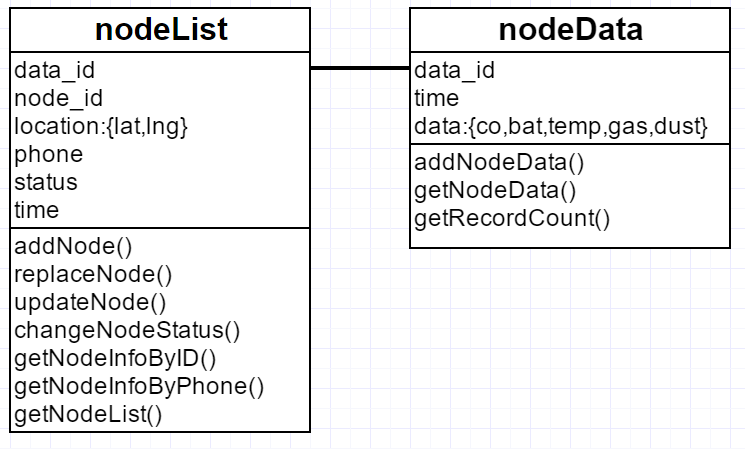
\includegraphics[width=1.0\textwidth]{dbnode}
	\caption[Mô hình cấu trúc dữ liệu của Sensor Node]{Mô hình cấu trúc dữ liệu của Sensor Node}
	\label{fig: dbnode}
\end{figure}
Về phía user, chỉ có một bảng quản lý người dùng bao gồm các thông tin cơ bản để xác thực và quyền thay đổi chỉnh sửa dữ liệu sensor node.
\begin{figure}[H]
	\centering    
	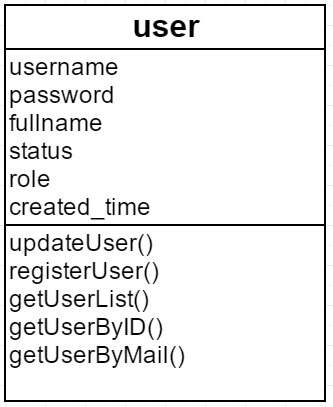
\includegraphics[width=0.45\textwidth]{dbuser}
	\caption[Mô hình cấu trúc dữ liệu của User]{Mô hình cấu trúc dữ liệu của User}
	\label{fig: dbuser}
\end{figure}

Vì mục hệ thống phát triển dừng ở mức xây dựng và thiết kế hệ thống thu thập và truy vấn dữ liệu từ các sensor node nên chưa có bảng phân quyền sở hữu giữa người dùng và sensor node.
\subsection{Hiện thực API}
Dựa trên mô hình thiết kế API tại \ref{sec: api}, API được hiện thực và phát triển.


\subsubsection*{API đăng ký và xác thực người dùng}

Các API này được xây dựng để quản lý và phân quyền người dùng, cho phép sử dụng các API về quản lý thông tin của các sensor node.

\textbf{Đăng nhập:}

Hệ thống sử dụng module Passport chạy trên nền Nodejs, có chức năng dễ dàng thiết lập xác thực người dùng. Module này có thể liên kết với các tài khoản phổ biến như Facebook, Google, Twitter... để hỗ trợ phương thức đăng nhập tiện lợi nhất cho người dùng. Tuy nhiên hệ thống chỉ sử dụng phương thức đăng nhập và quản lý người dùng ở mức local vì là phương thức phù hợp với đề tài.

Chi tiết API đăng nhập:
\begin{Verbatim}[xleftmargin=2em]
POST: /auth/login
data: {username,password}
RESPOND:
case Success:
	{
		code: 1,
		username,
		message: 'Login successful'
	}
case Failure	
	{
		code: 0,
		message: "Invalid username or password"
	}
======================
\end{Verbatim}

\textbf{Lưu thông tin người dùng bằng session:}

Sau khi đăng nhập, một session, còn gọi là phiên làm việc, sẽ được hình thành và lưu trữ trong thời gian nhất định. Session cho phép người dùng có thể vào các trang quản lý với quyền hạn cho phép mà không yêu cầu đăng nhập lại, cũng như được phép sử dụng các API quản lý sensor node.

Session sẽ tự động xóa sau một thời gian quy định, cụ thể ở hệ thống này là 10 ngày kể từ lần đăng nhập gần nhất. Người dùng có thể xóa thủ công bằng cách đăng xuất qua phương thức:
\begin{Verbatim}[xleftmargin=2em]
GET: /auth/logout
\end{Verbatim}

\textbf{Đăng ký:}

\begin{Verbatim}[xleftmargin=2em]
POST: /user/register
	data:{username, password, name, mail}
======================	
RESPOND:
	{
		code: -1,
		message: "Username existed"
	}
	{
		code: -2,
		message: "Mail is used",
	}
	{
		code: 1,
		message: "Account created successful"
	}
======================	
\end{Verbatim}
\subsubsection*{API cung cấp và quản lý sensor node}
Các API được miêu tả tại bảng \ref{table: apilist}, các request và respond được miêu tả chi tiết:

• API thiết lập và cấu hình các sensor node: initnew, updatenode và replace node yêu cầu phải có đăng nhập từ API xác thực người dùng để giữ session và sau đó mới có thể sử dụng. Các API này có cấu trúc tương tự nhau và được mô tả:
\begin{Verbatim}[xleftmargin=2em]
POST: /node/initnew
data: {node\_id,lat,lng,phone,status}
======================
RESPOND:
case Success:
	{
		code: 1,
		message: 'Add node successful'
	}
case Duplicated:
	{
		code: 0,
		message: 'Node duplicated'
	}
case Failure:
	{
		code: 0,
		message: 'Add node failure'
	}
case Not authenticated:
	{
		code: -1,
		message: 'You are not authenticated'
	}
======================	
\end{Verbatim}

• API get thông tin và dữ liệu các sensor node: sử dụng phương thức GET để truy xuất dữ liệu về thông tin sensor node và dữ liệu các cảm biến. Hệ thống được thiết kế mang tính mở và chia sẻ nên không yêu cầu đăng nhập để truy xuất dữ liệu. Các thông tin đặc tả chi tiết API:
\begin{Verbatim}[xleftmargin=2em]
GET:	/node/getinfo?*query
Ex: 	/node/getinfo?id=1&status=0
	    /node/getinfo?list=1&status=1
Query:
+ id=*node ID* để get node bằng ID
+ phone: *node phonenumber* để get node bằng phone number
+ list=1 để get list các node
+ status=1 để get node đang ở trạng thái active,= 0 để node ở tất cả 
trạng thái, cũng như lịch sử thay đổi node
======================
RESPOND:
data:
- single node:{node_id,location:{lat,lng},phone,,time,data_id,status}
- list: array of {node_id,location:{lat,lng},phone,time,data_id,status}
======================
\end{Verbatim}

• API push dữ liệu từ sensor node: cũng tương tự như API get dữ liệu, API push dữ liệu sử dụng method GET thay cho POST để hỗ trợ dễ dàng trong việc thiết lập các thiết bị IoT đóng góp dữ liệu. Lượng dữ liệu của các sensor node không quá lớn, chỉ bao gồm những trường sensor ID và node ID nên có thể tích hợp vào thanh header của request.

\begin{Verbatim}[xleftmargin=2em]
GET: 	/node/pushdata?*query
Ex: 	/node/pushdata?node_id=1&s1=22&s2=33&s3=44&s4=55&s5=66
Query:
+ node_id: node ID
+ s1,s2,s3,s4,s5: value of each sensor
======================
RESPOND:
case Success:
	{
		code: 1,
		message: 'Add node data successful'
	}
case Failure:	
	{
		code: 0,
		message: 'Add node data failure'
	}
======================
\end{Verbatim}

\subsubsection*{Cung cấp API log}

Để hỗ trợ bên nhà phát triển thứ ba ứng dụng API tốt hơn, hệ thống có cung cấp các thông tin hoạt động của server, các request và respond cũng như các dữ liệu được truy vấn. Khi truy cập vào đường dẫn /log/, chúng ta sẽ có những file log tương ứng với các ngày như hình \ref{fig: log} :

\begin{figure}[H]
	\centering    
	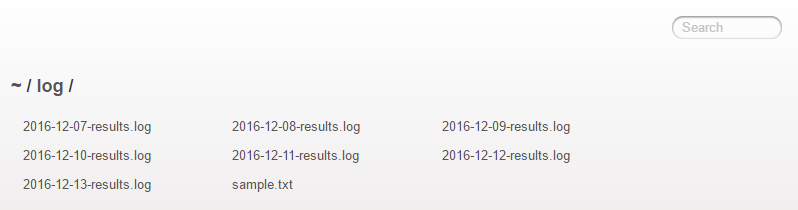
\includegraphics[width=1.0\textwidth]{log}
	\caption[Hiển thị các file log]{Hiển thị các file log}
	\label{fig: log}
\end{figure}

Ví dụ cụ thể của một đoạn log:
\begin{lstlisting}
{"level":"info","message":"IP:123.151.42.61 GET /route","timestamp":"10:48:56"}
{"level":"info","message":"IP:14.161.14.94 GET /statis route","timestamp":"10:49:22"}
{"level":"info","message":"IP:14.161.14.94 GET /graph route","timestamp":"10:49:27"}
{"level":"info","message":"IP:14.161.14.94 GET /node/getinfo: get list node info - number of nodes 12","timestamp":"10:49:27"}
{"level":"info","message":"IP:14.161.14.94 GET /node/getinfo: get node info by id:9","timestamp":"10:49:29",{"data_id":"106c59fe-753d-4a76-8418-88fd0df68d0c","id":"87b7f859-8c1e-4608-9645-5105ebb38e9b", "location":{"lat":10.91085286140159,"lng":106.99790954589844}, "node_id":"9","phone":"0123456899","status":1,"time":"2016-12-06T02:08:57.943Z"}}
{"level":"info","message":"IP:14.161.14.94 GET /node/getdata: Node data ID 9 number of records:  120","timestamp":"10:49:29"}
\end{lstlisting}

Các thông tin được thể hiện trong file log đủ thông tin để cho phép nhà phát triển theo dõi và áp dụng trong việc hiện thực sản phẩm.
\subsection{Xây dựng Web Server}

\subsection{Hiện thực giao diện}

Sử dụng framework express của Nodejs và HTML để xây dựng frontend

\subsubsection*{Giao diện chính của Web Server}
Phần này chứa các nút menu chức năng cùng với google map để theo dõi vị trí hoạt động của các cảm biến.
\begin{center}
\begin{figure}[H]
\centering    
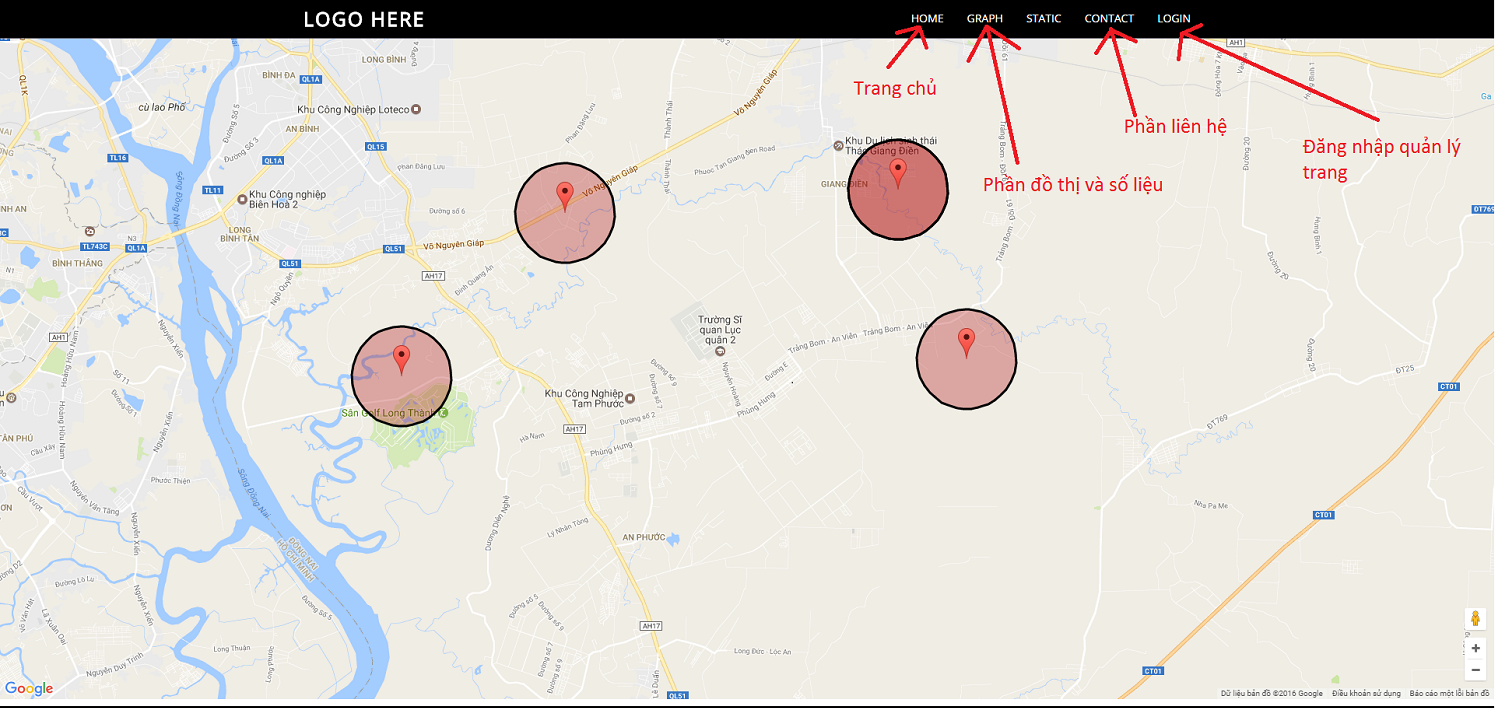
\includegraphics[width=1\textwidth]{webserver}
\caption[Giao diện chính của Web Server]{Giao diện chính của Web Server}
\label{fig:webserver}
\end{figure}
\end{center}

\subsubsection*{Giao diện đồ thị dữ liệu}
Là nơi hiện thị biểu đồ của các thông số cũng như thông tin tương ứng của các cảm biến.
\begin{center}
\begin{figure}[H]
\centering    
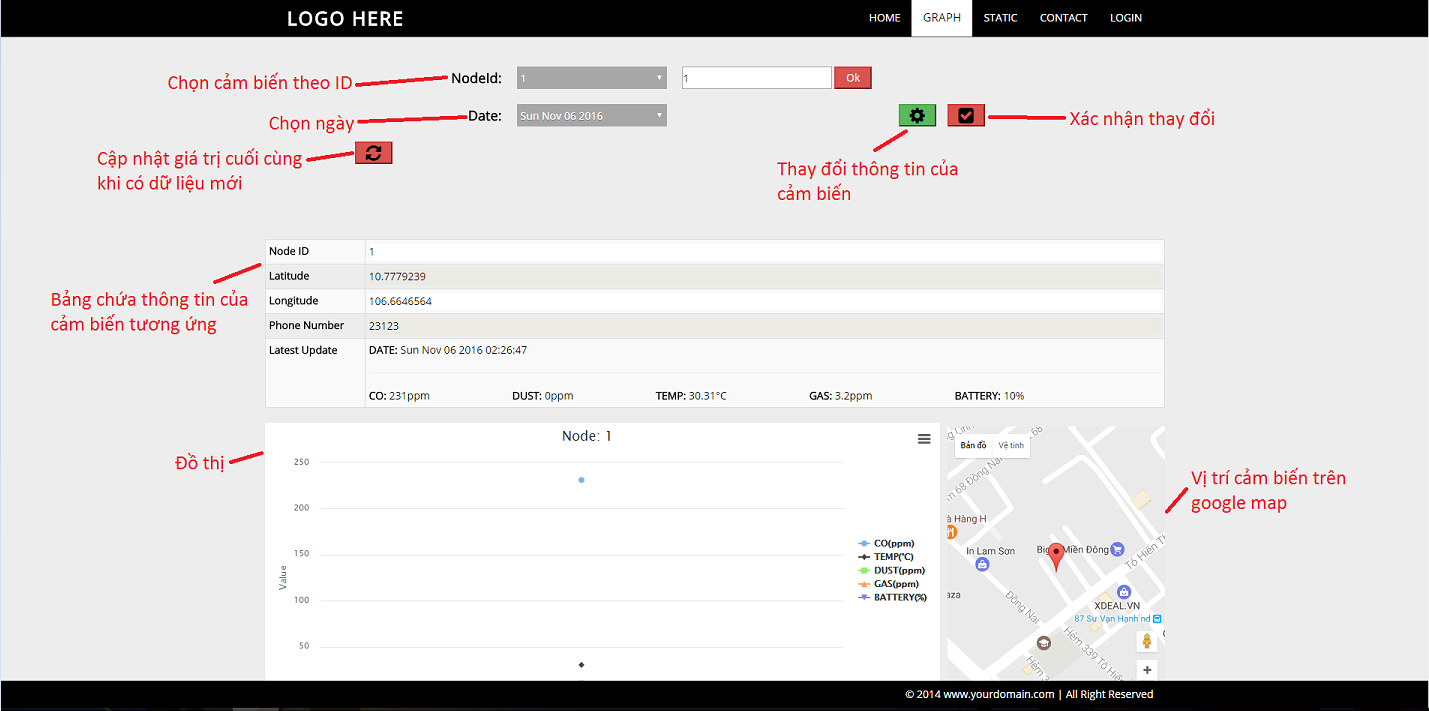
\includegraphics[width=1\textwidth]{web_graph}
\caption[Giao diện đồ thị dữ liệu]{Giao diện đồ thị dữ liệu}
\label{fig:web_graph}
\end{figure}
\end{center}



\subsubsection*{Giao diện nhận feedback từ người dùng qua email}
Tương tác giữa người dùng với người quản lý server. Nội dung được gửi thông qua gmail.
\begin{center}
\begin{figure}[H]
\centering    
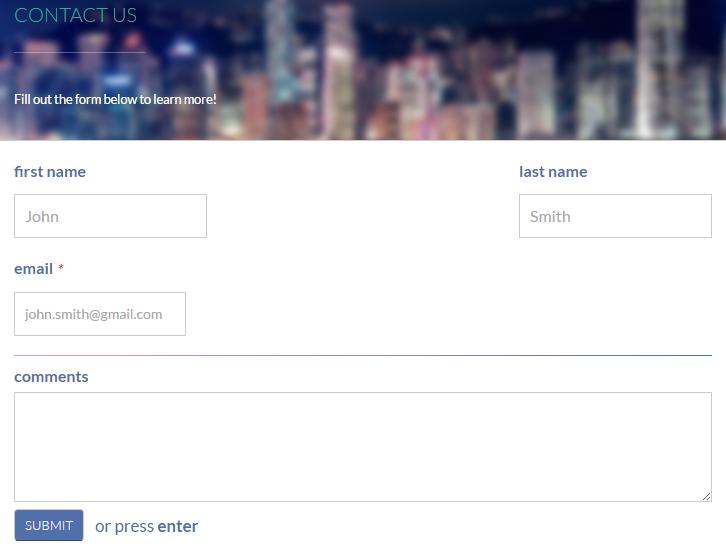
\includegraphics[width=1\textwidth]{web_email}
\caption[Giao diện nhận feedback người dùng]{Giao diện nhận feedback người dùng}
\label{fig:web_email}
\end{figure}
\end{center}

\subsubsection*{Giao diện dành cho người quản lý}
Khu vực này dành cho người quản lý truy cập nhầm mục đích chỉnh sửa, thay thế các node cảm biến.
\begin{center}
\begin{figure}[H]
\centering    
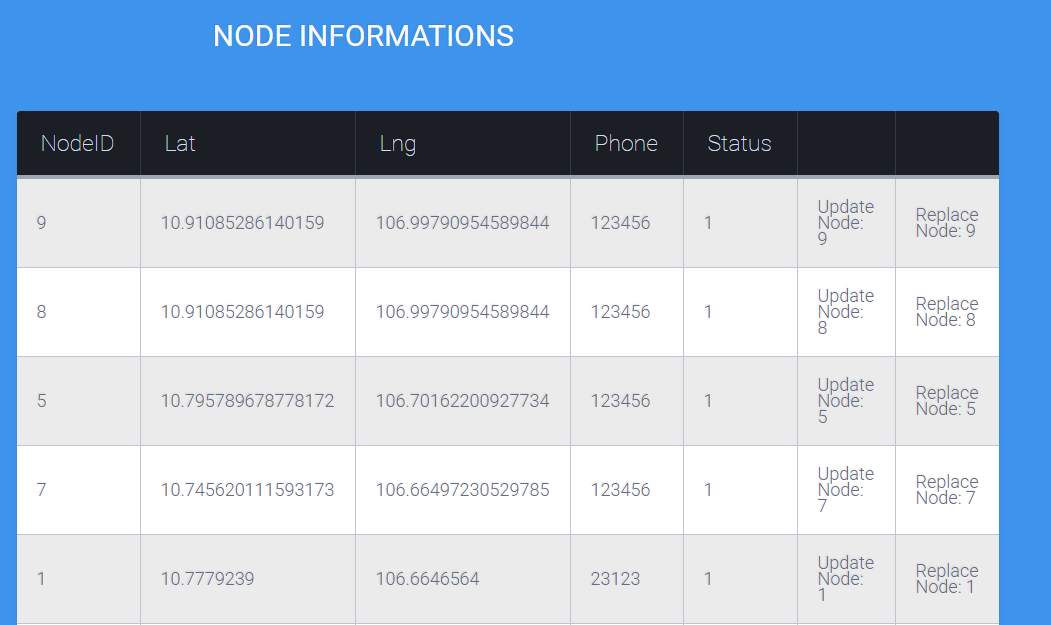
\includegraphics[width=1\textwidth]{web_nodeinfo}
\caption[Giao diện quản lý các node cảm biến]{Giao diện quản lý các node cảm biến}
\label{fig:web_nodeinfo}
\end{figure}
\end{center}
\section{Ứng dụng thiết bị di động}
\subsection{Hiện thực giao diện và chức năng}
\subsubsection*{Giao diện chính ứng dụng di động}
Tại giao diện chính của ứng dụng di động người dùng có thể xem được danh sách thông tin chi tiết của các node cảm biến có trong hệ thống.
\begin{center}
\begin{figure}[H]
\centering    
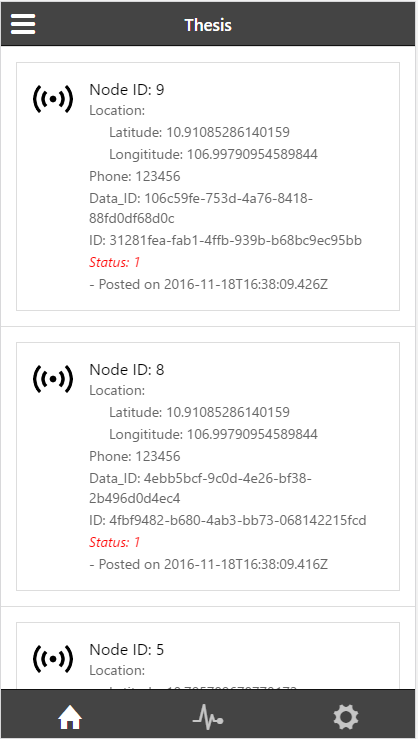
\includegraphics[width=0.4\textwidth]{app_main}
\caption[Giao diện chính ứng dụng di động]{Giao diện chính ứng dụng di động}
\label{fig:app_main}
\end{figure}
\end{center}


\subsubsection*{Giao diện xem dữ liệu trên ứng dụng di động}
Giao diện này cho phép người dùng theo dõi được dữ liệu của từng node cảm biến theo 2 loại biểu đồ như Hình \ref{fig:app_graph} thể hiện.
\begin{center}
\begin{figure}[H]
\centering    
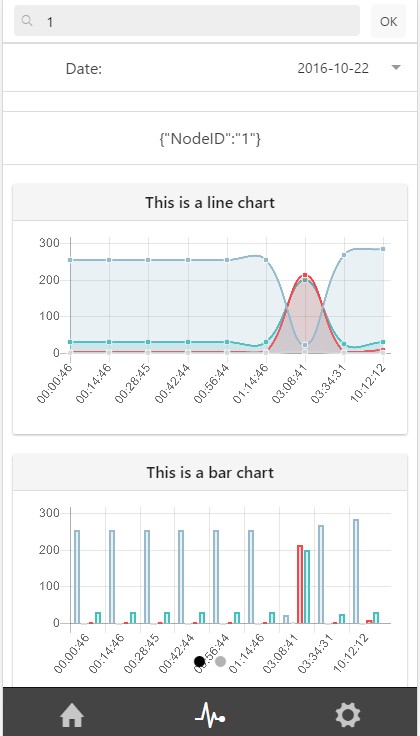
\includegraphics[width=0.4\textwidth]{app_graph}
\caption[Giao diện xem dữ liệu trên ứng dụng di động]{Giao diện xem dữ liệu trên ứng dụng di động}
\label{fig:app_graph}
\end{figure}
\end{center}


